\section{CAPÍTULO V: RESULTADOS}\label{cap:results}

\subsection{Estructura de los Resultados}\label{sec:results}

En este capítulo se presentan los resultados de la investigación mostrada en Metodología~\ref{cap:methodology}{color{red} Ojo que no sale la referencia cruzada. Lo he corregido}. Se ha dividido en dos partes, la primera muestra los resultados del Estudio 1 y la segunda los resultados del Estudio 2.

\subsection{Resultados del Estudio 1}\label{sec:resultados-estudio-1}

\subsubsection{Frecuencia Cardíaca}

A continuación, se muestra el análisis de la varianza realizado para la \textit{Frecuencia Cardíaca}, la \textit{Frecuencia Cardíaca Escalada} y la \textit{Frecuencia Cardíaca Transformada por Cuantiles} entre pacientes que sufren DETERIORO y los que no. Se ha realizado el análisis de la varianza para cada una de las medias horarias. El resultado se muestra en la Tabla~\ref{tab:mean-FC}.  


\begin{table}[H]
    \centering
    \begin{tabular}{|c|r|r|r|}
        \hline
        \textbf{Media Horaria} & \textbf{p-valor} & \textbf{p-valor 
        cuantiles} & \textbf{p-valor 
        escalada} \\
        \hline
        MEAN\_1 & 0.129 & 0.142 & 0.902 \\
        MEAN\_2 & 0.254 & 0.412 & 0.825 \\
        MEAN\_3 & 0.143 & 0.105 & 0.925 \\
        MEAN\_4 & 0.331 & 0.309 & 0.867 \\
        MEAN\_5 & 0.077 & 0.042 & 0.355 \\
        MEAN\_6 & 0.098 & 0.1 & 0.5 \\
        MEAN\_7 & 0.357 & 0.232 & 0.474 \\
        MEAN\_8 & 0.182 & 0.218 & 0.975 \\
        MEAN\_9 & 0.158 & 0.241 & 0.83 \\
        MEAN\_10 & 0.316 & 0.423 & 0.211 \\
        MEAN\_11 & 0.609 & 0.637 & 0.045 \\
        MEAN\_12 & 0.035 & 0.005 & 0.382 \\
        MEAN\_13 & 0.293 & 0.144 & 0.603 \\
        MEAN\_14 & 0.169 & 0.17 & 0.727 \\
        MEAN\_15 & 0.214 & 0.335 & 0.722 \\
        MEAN\_16 & 0.094 & 0.136 & 0.652 \\
        MEAN\_17 & 0.127 & 0.132 & 0.943 \\
        MEAN\_18 & 0.476 & 0.816 & 0.56 \\
        MEAN\_19 & 0.128 & 0.086 & 0.731 \\
        MEAN\_20 & 0.2 & 0.186 & 0.947 \\
        MEAN\_21 & 0.391 & 0.592 & 0.643 \\
        MEAN\_22 & 0.157 & 0.198 & 0.875 \\
        MEAN\_23 & 0.1 & 0.026 & 0.445 \\
        MEAN\_24 & 0.204 & 0.187 & 0.95 \\
        \hline
    \end{tabular}
    \caption{p-valor de la media horaria de la \textit{Frecuencia Cardíaca} y la \textit{Frecuencia Cardíaca Transformada por Cuantiles} entre pacientes que sufren OAF y los que no}\label{tab:mean-FC}
\end{table}

De manera gráfica el resultado es el siguiente mostrado en la Figura~\ref{fig:mean-FC}. Se han añadido dos rectas verticales que muestran el nivel del valor $\alpha$ = 0.05 y $\alpha$ = 0.001. ($\alpha$ = 0.01 se excluye del gráfico ya que a pesar de ser un nivel de significancia ampliamente utilizado, haría que el gráfico se viese peor al amontonarse las líneas verticales en la parte inferior de la imagen). Se puede observar que la mayoría de las medias horarias no son significativas, por lo que no se puede rechazar la hipótesis nula. Esto significa que no hay diferencias significativas entre las medias horarias de la \textit{Frecuencia Cardíaca} entre pacientes que sufren DETERIORO y los que no.

Se puede observar como de manera general que a los pacientes que se les suministra OAF tienen una mayor \textit{Frecuencia Cardíaca} que los que no. Esto se puede observar en la Figura~\ref{fig:fc-boxplot-mean}, aun así no se puede afirmar que esto tenga un efecto significativo de manera general en toda la monitorización del paciente.

Las medias más significativas son las referentes a las horas 12 y 23. Esta situación va a causar a la hora de realizar el \textit{Estudio 2} se tendrán problemas a la hora de realizar un modelo de clasificación dónde los valores de monitorización de la \textit{Frecuencia Cardíaca} sean significativos a la hora de clasificar pacientes como DETERIORO o no.

\begin{figure}[H]
    \centering
    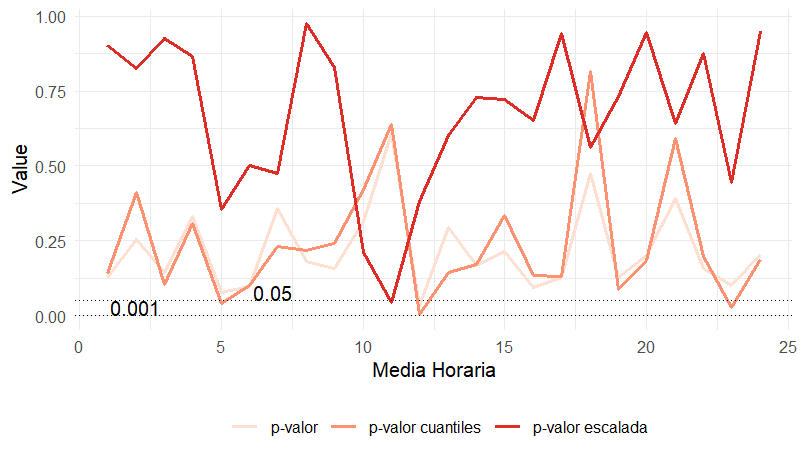
\includegraphics[scale = 1]{./img/mean-FC.png}
    \caption{p-valor de la media horaria de la \textit{Frecuencia Cardíaca} entre pacientes que sufren DETERIORO y los que no}
    \label{fig:mean-FC}
\end{figure}

\newpage
\thispagestyle{empty}
% Se modifica la geometría (los márgenes) de la página y se coloca en formato horizontal:
\newgeometry{top=10mm, bottom=10mm, left=12mm, right=12mm}
\begin{landscape}
\begin{figure}[H]
    \centering
    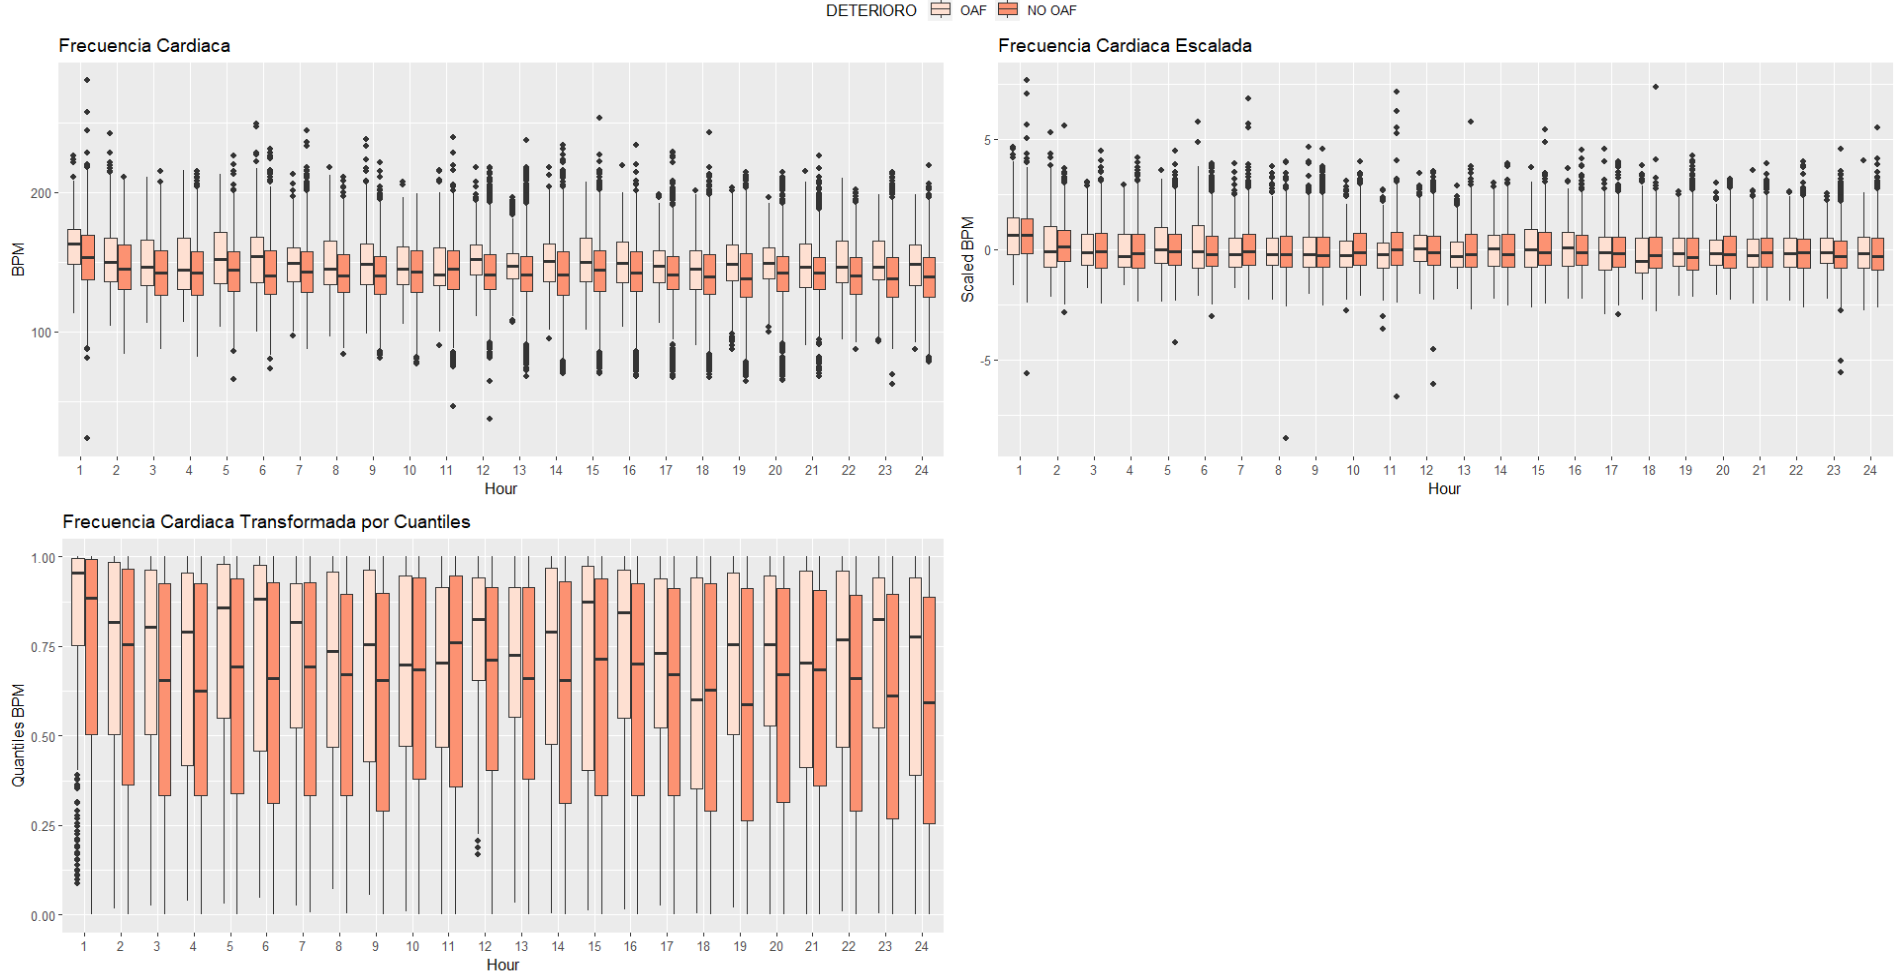
\includegraphics[scale = 0.68]{./img/fc-boxplot-mean.png}
    \caption{Media Horaria de la \textit{Frecuencia Cardíaca}, \textit{Frecuencia Cardíaca Escalada} y la \textit{Frecuencia Cardíaca Transformada por Cuantiles} entre pacientes que sufren DETERIORO y los que no}
    \label{fig:fc-boxplot-mean}
\end{figure}
\end{landscape}
\restoregeometry

\subsubsection{Saturación de Oxígeno}

A continuación, se muestra el análisis de la varianza realizado para la \textit{Saturación de O$_2$} y la \textit{Saturación de O$_2$ Escalada} entre pacientes que sufren DETERIORO y los que no. Se ha realizado el análisis de la varianza para cada una de las medias horarias. El resultado se muestra en la Tabla~\ref{tab:mean-SatO2}.

\begin{table}[H]
    \centering
    \begin{tabular}{|c|r|r|}
        \hline
        \textbf{Media Horaria} & \textbf{p-valor} & \textbf{p-valor escalada} \\
        \hline
        MEAN\_1 & 0.151 & 0.176 \\
        MEAN\_2 & 0.015 & 0.017 \\
        MEAN\_3 & 0.52 & 0.778 \\
        MEAN\_4 & 0.343 & 0.608 \\
        MEAN\_5 & 0.349 & 0.718 \\
        MEAN\_6 & 0.672 & 0.639 \\
        MEAN\_7 & 0.141 & 0.078 \\
        MEAN\_8 & 0.868 & 0.769 \\
        MEAN\_9 & 0.571 & 0.939 \\
        MEAN\_10 & 0.549 & 0.842 \\
        MEAN\_11 & 0.991 & 0.643 \\
        MEAN\_12 & 0.44 & 0.581 \\
        MEAN\_13 & 0.312 & 0.427 \\
        MEAN\_14 & 0.968 & 0.797 \\
        MEAN\_15 & 0.641 & 0.966 \\
        MEAN\_16 & 0.799 & 0.183 \\
        MEAN\_17 & 0.312 & 0.993 \\
        MEAN\_18 & 0.89 & 0.204 \\
        MEAN\_19 & 0.543 & 0.71 \\
        MEAN\_20 & 0.384 & 0.784 \\
        MEAN\_21 & 0.867 & 0.503 \\
        MEAN\_22 & 0.665 & 0.195 \\
        MEAN\_23 & 0.882 & 0.294 \\
        MEAN\_24 & 0.889 & 0.358 \\
        \hline
    \end{tabular}
    \caption{p-valor de la media horaria de la \textit{Saturación de O$_2$} entre pacientes que sufren OAF y los que no}\label{tab:mean-SatO2}
\end{table}

Al igual que en el apartado anterior el resultado es el siguiente mostrado en la Figura~\ref{fig:mean-SatO2}. La mayoría de las medias horarias no son significativas, por lo que no se puede rechazar la hipótesis nula. Esto significa que no hay diferencias significativas entre las medias horarias de la \textit{Saturación de O$_2$} entre pacientes que sufren DETERIORO y los que no.

Se puede observar como de manera general que a los pacientes que se les suministra OAF tienen una mayor \textit{Saturación de O$_2$} que los que no. Esto se puede observar en la Figura~\ref{fig:satO2-boxplot-mean}, aun así no se puede afirmar que esto tenga un efecto significativo de manera general en toda la monitorización del paciente.

La única media significativa menor que $\alpha = 0.05$ es la monitorizada en la hora $2$. Al igual que en el apartado anterior, esta situación va a causar a la hora de realizar el \textit{Estudio 2} se tendrán problemas a la hora de realizar un modelo de clasificación dónde los valores de monitorización de la \textit{Saturación de O$_2$} sean significativos a la hora de clasificar pacientes como DETERIORO o no.

\begin{figure}[H]
    \centering
    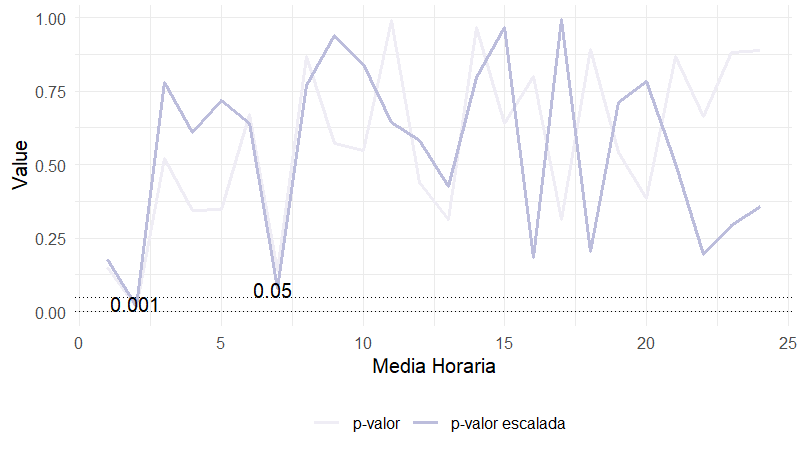
\includegraphics[scale = 1]{./img/mean-SatO2.png}
    \caption{p-valor de la media horaria de la \textit{Saturación de Oxígeno} entre pacientes que sufren DETERIORO y los que no}
    \label{fig:mean-SatO2}
\end{figure}

\newpage
\thispagestyle{empty}
% Se modifica la geometría (los márgenes) de la página y se coloca en formato horizontal:
\newgeometry{top=10mm, bottom=10mm, left=12mm, right=12mm}
\begin{landscape}
\begin{figure}[H]
    \centering
    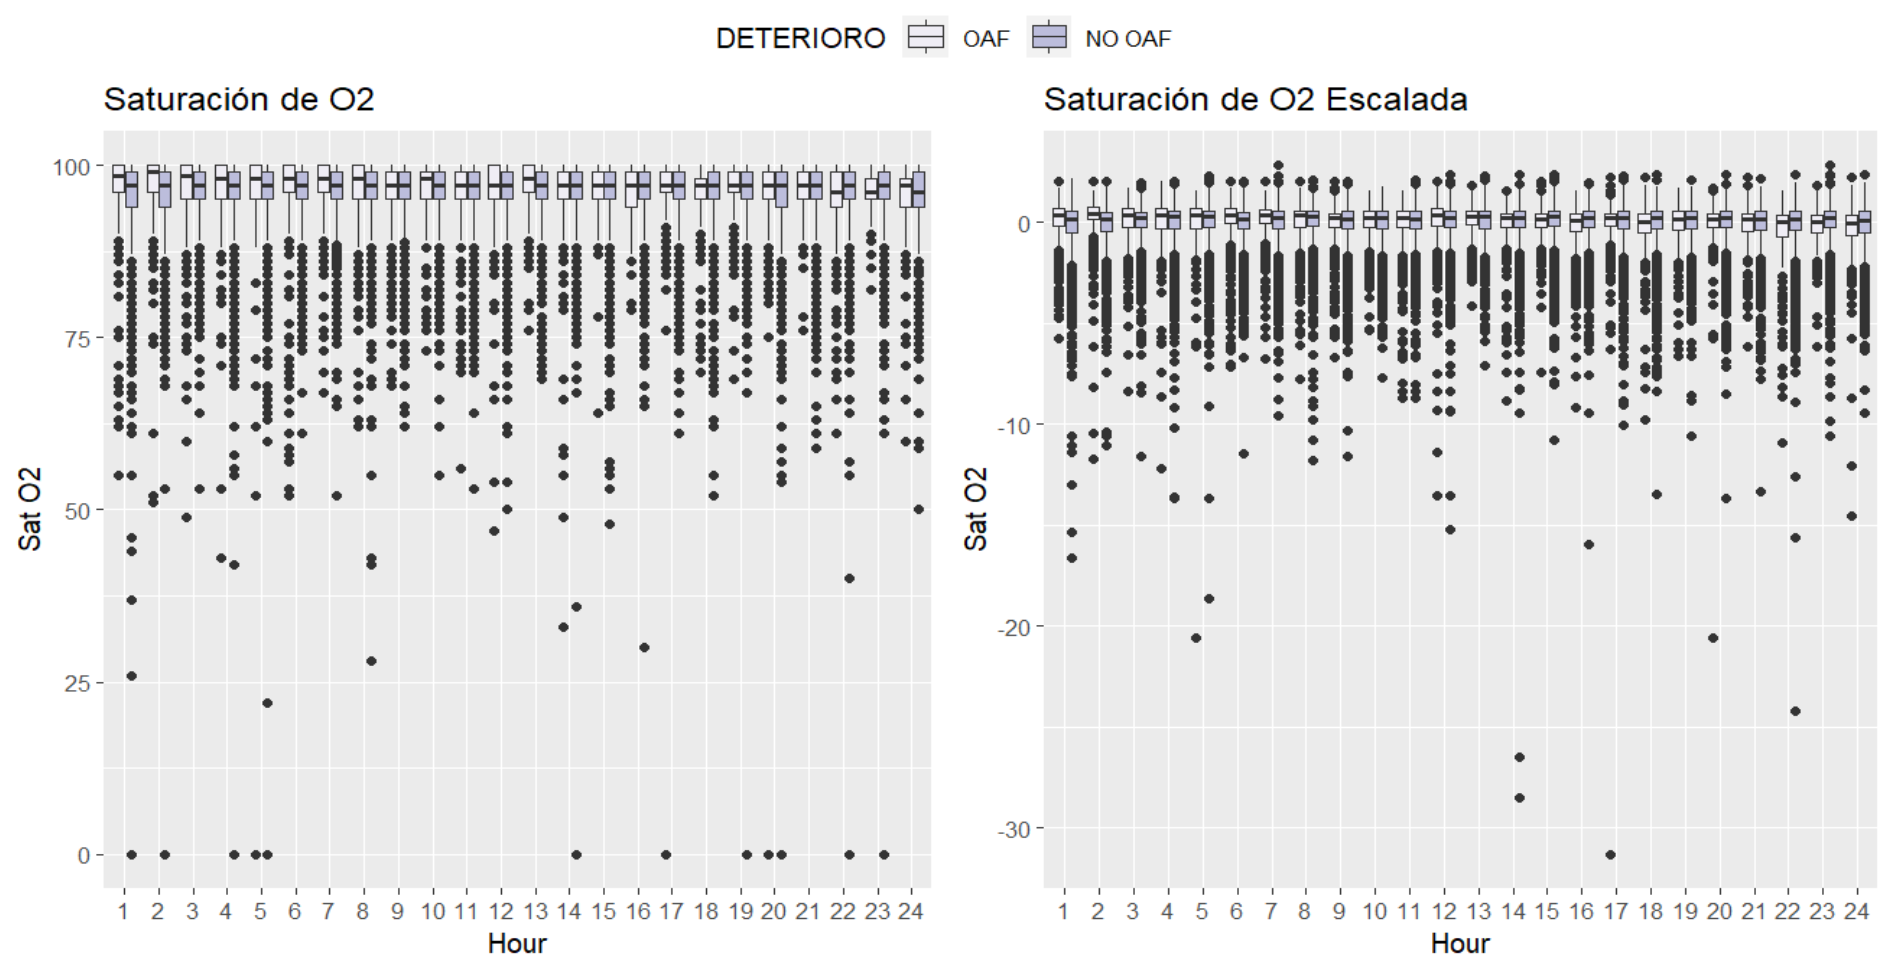
\includegraphics[scale = 0.68]{./img/satO2-boxplot-mean.png}
    \caption{Media Horaria de la \textit{Saturación de Oxígeno} y la \textit{Saturación de Oxígeno Escalada} entre pacientes que sufren DETERIORO y los que no}
    \label{fig:satO2-boxplot-mean}
\end{figure}
\end{landscape}
\restoregeometry


\subsection{Resultados: Estudio 2}\label{sec:resultados-estudio-1}

En esta sección de resultados, presentaremos los hallazgos obtenidos en el \textit{Estudio 2}. La sección se subdivide en cuatro subsecciones, y en cada una de ellas se mostrarán los siguientes resultados:

\begin{enumerate}
    \item Dendrograma de los clústeres obtenidos según la mejor agrupación determinada.
    \item Distribución de los clústeres obtenidos en función de las dos primeras componentes principales según la mejor agrupación determinada.
    \item Puntuación de Silhouette de los clústeres obtenidos según la mejor agrupación determinada.
    \item Dendrograma de los clústeres obtenidos según los pacientes que han experimentado OAF, junto con la tabla de contingencia para dos grupos de pacientes.
    \item Clasificación mediante Random Forest de los clústeres según las variables \textit{Cuantitativas} y \textit{Cualitativas} de la Tabla~\ref{tabla:variables_estudio_final}, así como la Importancia de las cinco primeras variables para dos grupos de pacientes.
    \item Clasificación Discriminante mediante Random Forest de los clústeres en función de los datos utilizados para generar los mismos clústeres (Raw Data, FAC, {\color{blue}Periodograma} y FACC). Se mostrará la importancia para identificar qué datos contribuyen más en la clasificación entre k = 2 clústers generados.
    \item Distribución de la importancia del resultado del modelo del apartado anterior de los valores empleados (Raw Data, FAC, {\color{blue}Periodograma} y FACC) 
    \item Cálculo de las medias de todos los valores empleados (Raw Data, FAC, {\color{blue}Periodograma} y FACC) entre todos los pacientes, y diagrama de sus valores entre k = 2 clústers generados.
\end{enumerate}

Se estudiará la mejor forma de distribuir a los pacientes entre clusters pero se tendrá en cuenta que al pretender dividir la muestra de pacientes entre aquellos a los que se les suministra  OAF y los que no{\color{blue},} {\color{red} esta coma es importante} se forzará para su clasificación y visualización a 2 clusters.

\paragraph{Leyenda de los gráficos}

\begin{enumerate}
    \item \textbf{Frecuencia Cardíaca}: \textit{HR}.
    \item \textbf{Saturación de Oxígeno}: \textit{SpO2}.
    \item \textbf{Frecuencia Cardíaca Escalada}: \textit{HR\_scaled}.
    \item \textbf{Saturación de Oxígeno Escalada}: \textit{SpO2\_scaled}.
    \item \textbf{Frecuencia Cardíaca Transformada por Cuantiles}: \textit{HR\_quantile}.
\end{enumerate}

\newpage
\subsubsection{Raw Data}

\paragraph{Dendrograma de los clústeres obtenidos}

\begin{figure}[H]
    \centering
    
    \subfigure[\textit{HR}]{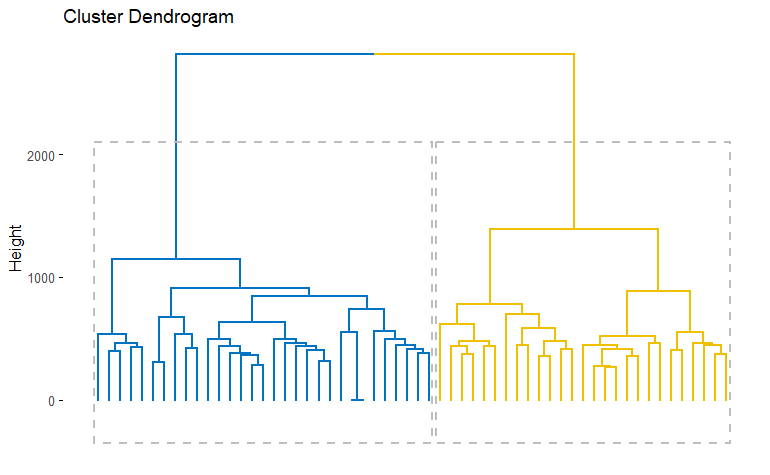
\includegraphics[width=0.45\textwidth]{img/01-1-eucl.png}}
    \subfigure[\textit{HR\_scaled}]{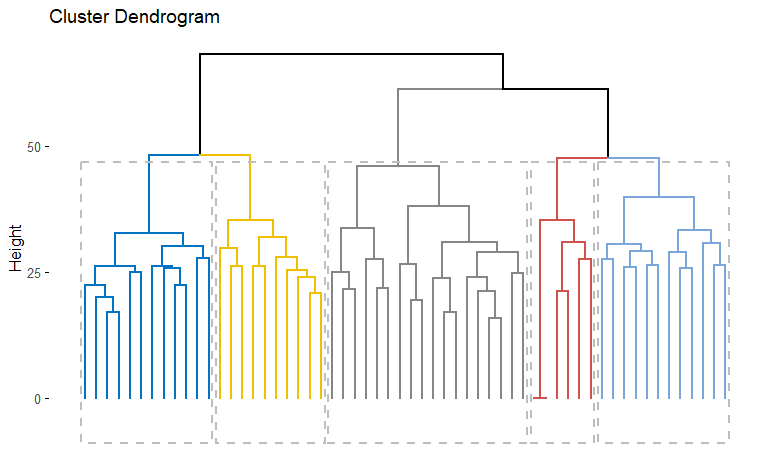
\includegraphics[width=0.45\textwidth]{img/02-1-eucl.png}}
    \subfigure[\textit{HR\_quantile}]{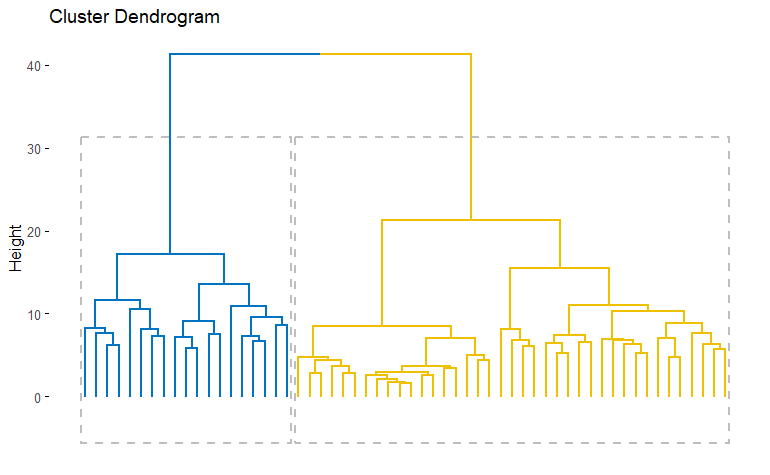
\includegraphics[width=0.5\textwidth]{img/03-1-eucl.png}}
    \caption{Dendogramas de \textit{HR}, \textit{HR\_scaled} y \textit{HR\_quantile}}
    \label{fig:raw_data_den_fc}
\end{figure}

\begin{figure}[ht]
    \centering
    \subfigure[\textit{SpO2}]{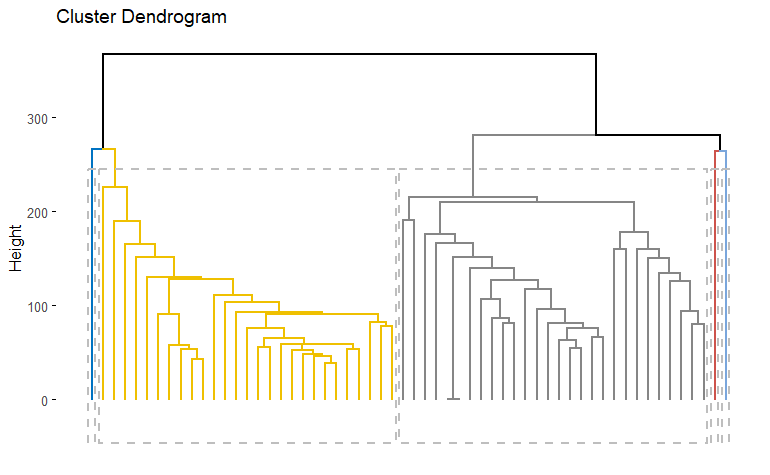
\includegraphics[width=0.5\textwidth]{img/04-1-eucl.png}}\hfill
    \subfigure[\textit{SpO2\_scaled}]{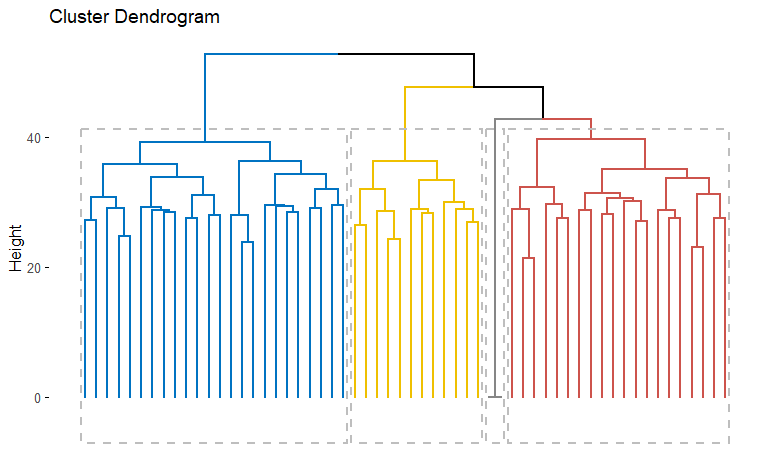
\includegraphics[width=0.5\textwidth]{img/05-1-eucl.png}}
    \caption{Dendogramas de \textit{SpO2} y \textit{SpO2\_scaled}}\label{fig:raw_data_den_spo2}
\end{figure}

\paragraph{Distribución de los clústeres obtenidos en función de las dos primeras componentes principales}

\begin{figure}[H]
    \centering
    \subfigure[\textit{HR}]{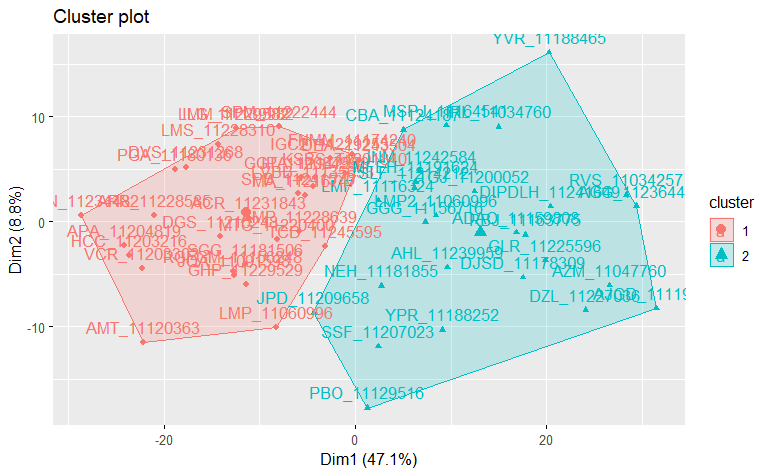
\includegraphics[width=0.45\textwidth]{img/01-2-eucl.png}}
    \subfigure[\textit{HR\_scaled}]{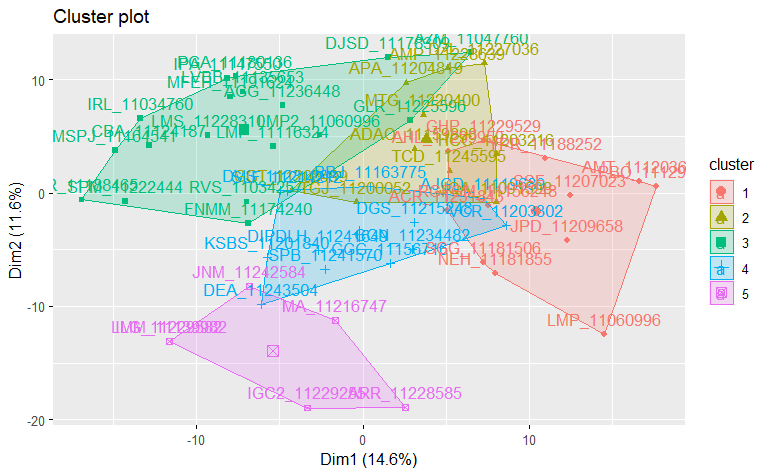
\includegraphics[width=0.45\textwidth]{img/02-2-eucl.png}}
    \subfigure[\textit{HR\_quantile}]{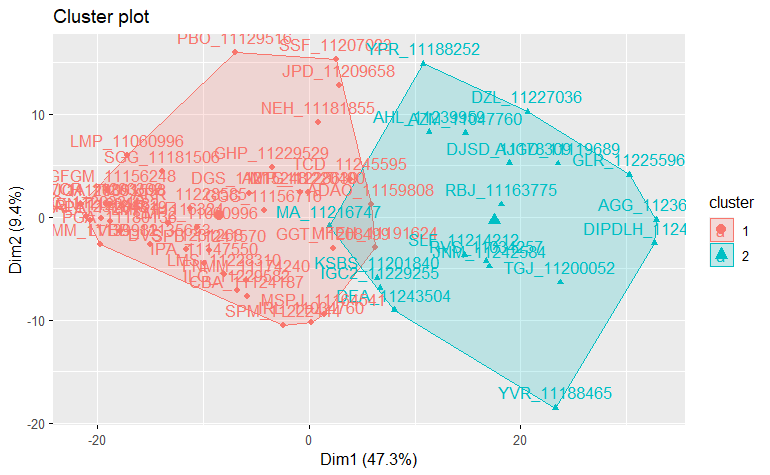
\includegraphics[width=0.5\textwidth]{img/03-2-eucl.png}}
    \caption{Cluster Plot de \textit{HR}, \textit{HR\_scaled} y \textit{HR\_quantile}}
    \label{fig:raw_data_pc_fc}
\end{figure}

\begin{figure}[ht]
    \centering
    \subfigure[\textit{SpO2}]{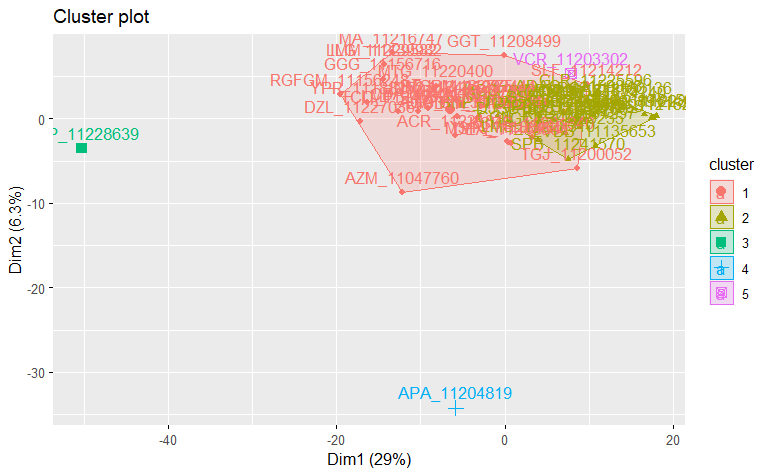
\includegraphics[width=0.5\textwidth]{img/04-2-eucl.png}}\hfill
    \subfigure[\textit{SpO2\_scaled}]{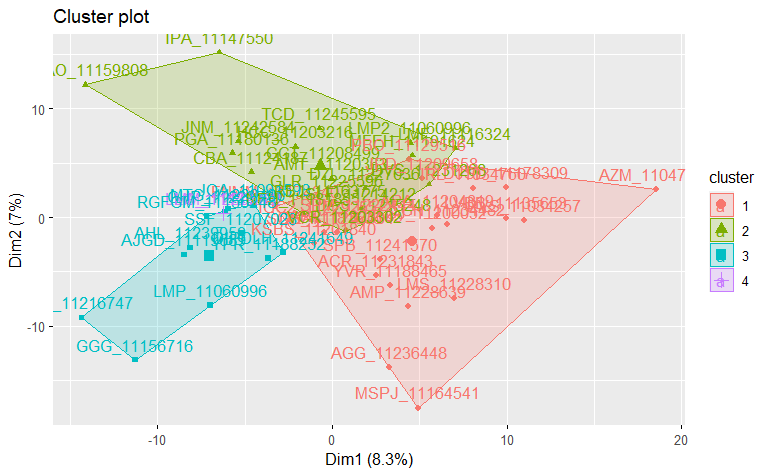
\includegraphics[width=0.5\textwidth]{img/05-2-eucl.png}}
    \caption{Cluster Plot de \textit{SpO2} y \textit{SpO2\_scaled}}\label{fig:raw_data_pc_spo2}
\end{figure}


\paragraph{Puntuación de Silhouette de los clústeres obtenidos}

\begin{figure}[H]
    \centering
    \subfigure[\textit{HR}]{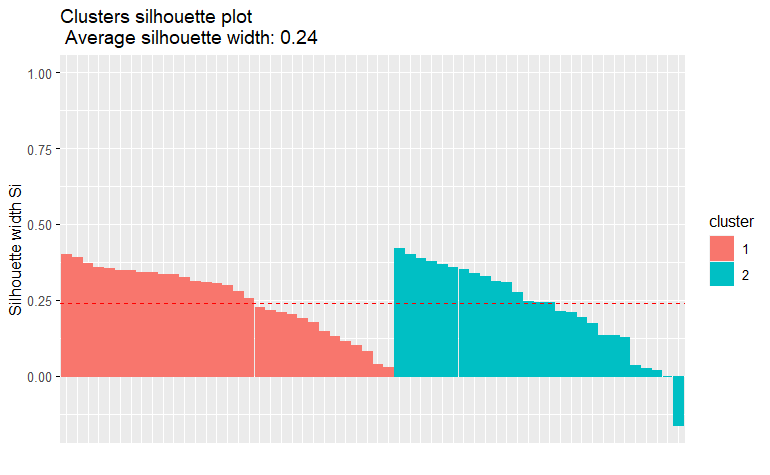
\includegraphics[width=0.45\textwidth]{img/01-3-eucl.png}}
    \subfigure[\textit{HR\_scaled}]{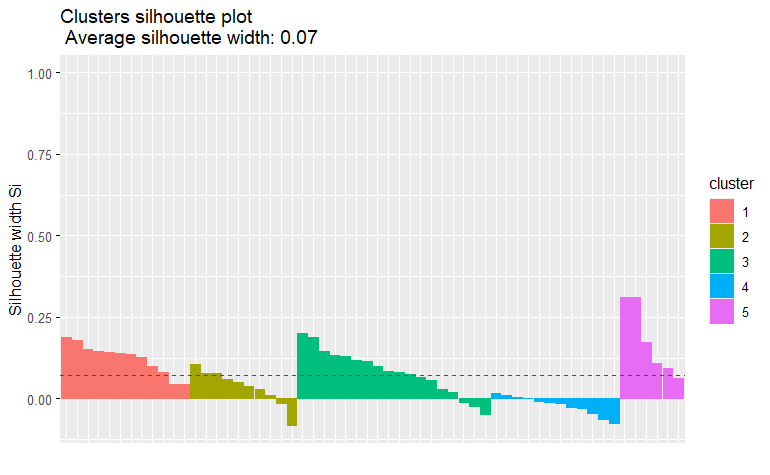
\includegraphics[width=0.45\textwidth]{img/02-3-eucl.png}}
    \subfigure[\textit{HR\_quantile}]{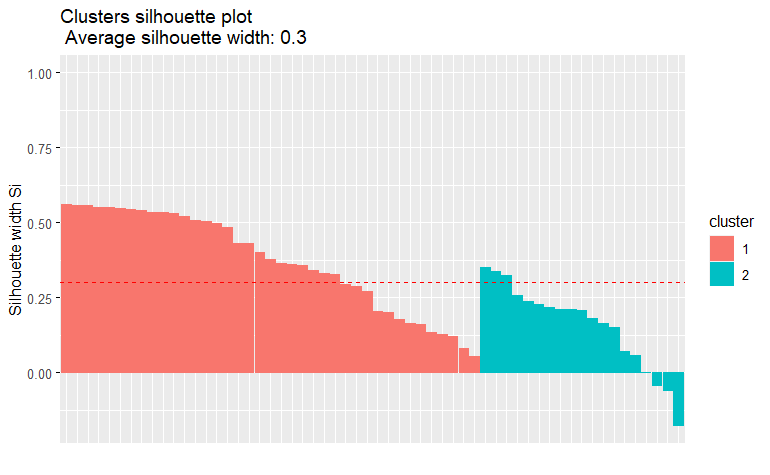
\includegraphics[width=0.5\textwidth]{img/03-3-eucl.png}}
    \caption{Silhouette Plot de \textit{HR}, \textit{HR\_scaled} y \textit{HR\_quantile}}\label{fig:raw_data_si_fc}
\end{figure}

\begin{figure}[ht]
    \centering
    \subfigure[\textit{SpO2}]{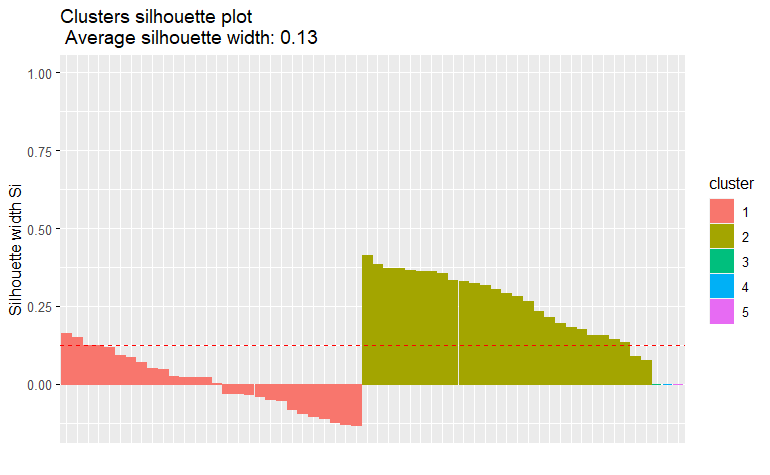
\includegraphics[width=0.5\textwidth]{img/04-3-eucl.png}}\hfill
    \subfigure[\textit{SpO2\_scaled}]{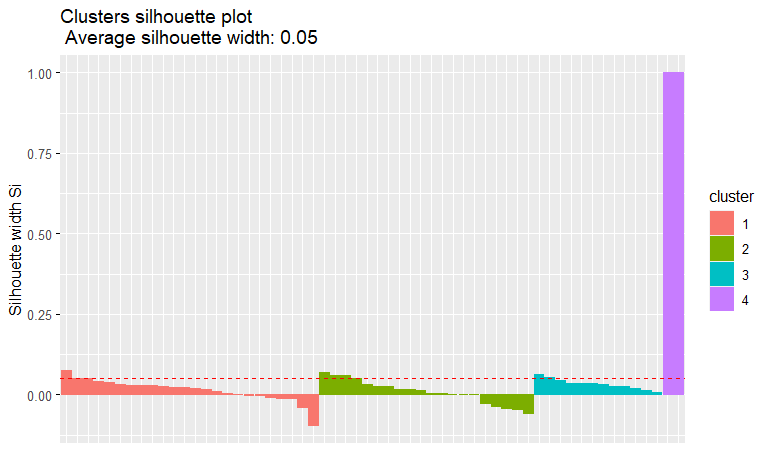
\includegraphics[width=0.5\textwidth]{img/05-3-eucl.png}}
    \caption{Silhouette Plot de \textit{SpO2} y \textit{SpO2\_scaled}}\label{fig:raw_data_si_spo2}
\end{figure}

\paragraph{Dendograma dividido en dos clústeres según los pacientes que han experimentado OAF}

\begin{figure}[H]
    \centering
    \subfigure[\textit{HR}]{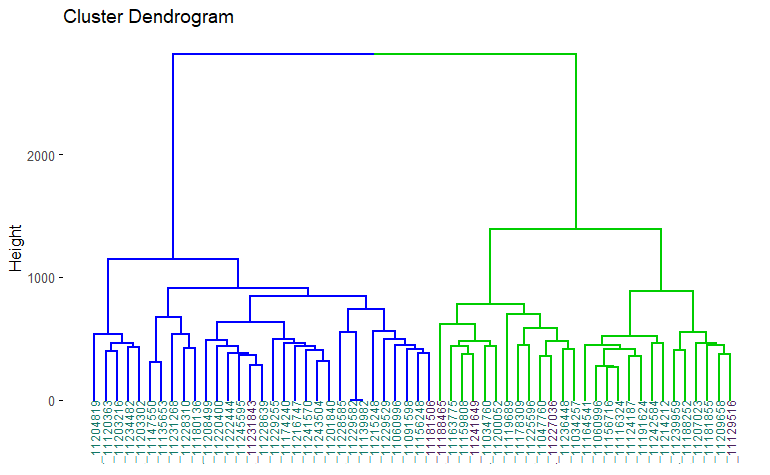
\includegraphics[width=0.45\textwidth]{img/01-4-eucl.png}}
    \subfigure[\textit{HR\_scaled}]{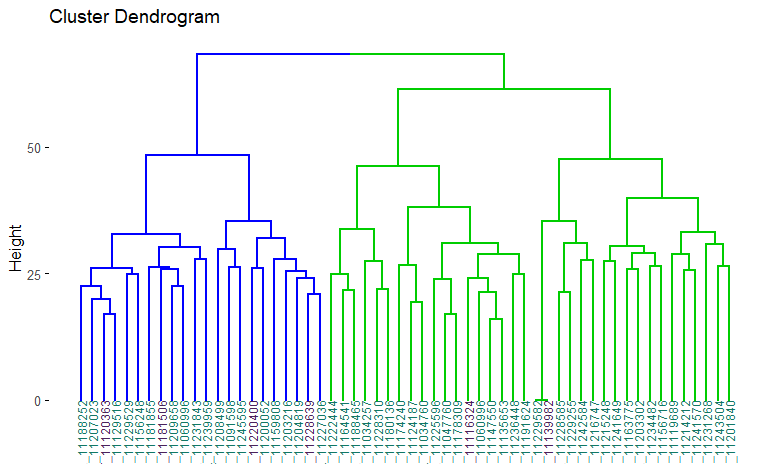
\includegraphics[width=0.45\textwidth]{img/02-4-eucl.png}}
    \subfigure[\textit{HR\_quantile}]{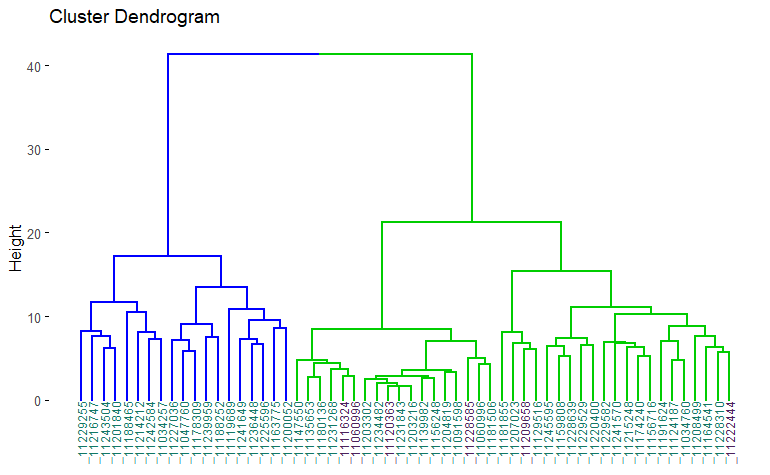
\includegraphics[width=0.5\textwidth]{img/03-4-eucl.png}}
    \caption{Dendograma Plot k = 2 de \textit{HR}, \textit{HR\_scaled} y \textit{HR\_quantile}}\label{fig:raw_data_ctg_fc}
\end{figure}

\begin{figure}[ht]
    \centering
    \subfigure[\textit{SpO2}]{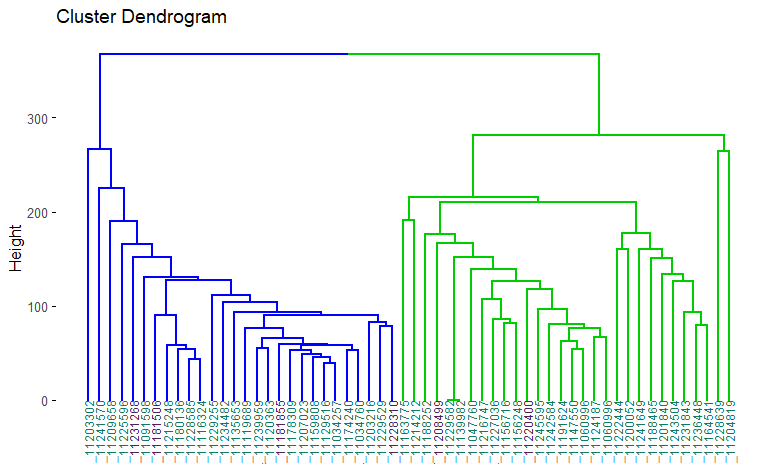
\includegraphics[width=0.5\textwidth]{img/04-4-eucl.png}}\hfill
    \subfigure[\textit{SpO2\_scaled}]{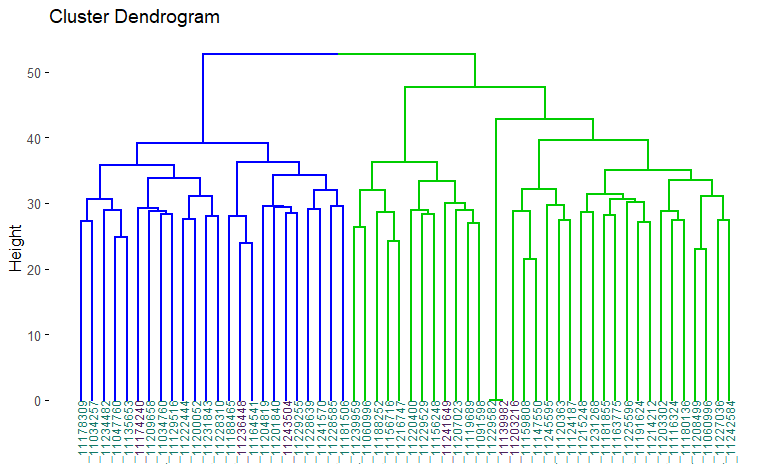
\includegraphics[width=0.5\textwidth]{img/05-4-eucl.png}}
    \caption{Dendograma Plot k = 2 de \textit{SpO2} y \textit{SpO2\_scaled}}\label{fig:raw_data_ctg_spo2}
\end{figure}

\paragraph{Clasificación mediente Random Forest de los clústeres según las variables \textit{Cuantitativas} y \textit{Cualitativas} de la Tabla~\ref{tabla:variables_estudio_final}}

\begin{figure}[H]
    \centering
    \begin{lstlisting}[frame=single, basicstyle=\small\ttfamily]
        randomForest(formula = CLUSTER ~ ., data = newSMOTE_EUCL) 
        Type of random forest: classification
              Number of trees: 500
No. of variables tried at each split: 5

 OOB estimate of  error rate: 39.66%
Confusion matrix:
1  2 class.error
1 19 12   0.3870968
2 11 16   0.4074074
    \end{lstlisting}
    \caption{Resultado de Random Forest para \textit{HR} utilizando variables \textit{Cuantitativas} y \textit{Cualitativas} de la Tabla~\ref{tabla:variables_estudio_final} y clasificación de clusters k = 2}\label{fig:random_forest_eucl_result_1}
\end{figure}
\begin{figure}[H]
    \centering
    \begin{lstlisting}[frame=single, basicstyle=\small\ttfamily]
        randomForest(formula = CLUSTER ~ ., data = newSMOTE_EUCL) 
               Type of random forest: classification
                     Number of trees: 500
No. of variables tried at each split: 5

        OOB estimate of  error rate: 43.1%
Confusion matrix:
  1  2 class.error
1 6 16   0.7272727
2 9 27   0.2500000
    \end{lstlisting}
    \caption{Resultado de Random Forest para \textit{HR\_scaled} utilizando variables \textit{Cuantitativas} y \textit{Cualitativas} de la Tabla~\ref{tabla:variables_estudio_final} y clasificación de clusters k = 2}
    \label{fig:random_forest_eucl_result_2}
\end{figure}

\begin{figure}[H]
    \centering
    \begin{lstlisting}[frame=single, basicstyle=\small\ttfamily]
        randomForest(formula = CLUSTER ~ ., data = newMWMOTE_EUCL) 
               Type of random forest: classification
                     Number of trees: 500
No. of variables tried at each split: 5

        OOB estimate of  error rate: 36.99%
Confusion matrix:
   1  2 class.error
1 26 13   0.3333333
2 14 20   0.4117647
    \end{lstlisting}
    \caption{Resultado de Random Forest para \textit{HR\_quantile} utilizando variables \textit{Cuantitativas} y \textit{Cualitativas} de la Tabla~\ref{tabla:variables_estudio_final} y clasificación de clusters k = 2}
    \label{fig:random_forest_eucl_result_3}
\end{figure}

\begin{figure}[H]
    \centering
    \begin{lstlisting}[frame=single, basicstyle=\small\ttfamily]
        randomForest(formula = CLUSTER ~ ., data = newSMOTE_EUCL) 
               Type of random forest: classification
                     Number of trees: 500
No. of variables tried at each split: 5

        OOB estimate of  error rate: 48.28%
Confusion matrix:
   1  2 class.error
1 16 14   0.4666667
2 14 14   0.5000000
    \end{lstlisting}
    \caption{Resultado de Random Forest para \textit{SpO2} utilizando variables \textit{Cuantitativas} y \textit{Cualitativas} de la Tabla~\ref{tabla:variables_estudio_final} y clasificación de clusters k = 2}\label{fig:random_forest_eucl_result_4}
\end{figure}
\begin{figure}[H]
    \centering
    \begin{lstlisting}[frame=single, basicstyle=\small\ttfamily]
        randomForest(formula = CLUSTER ~ ., data = newSMOTE_EUCL) 
               Type of random forest: classification
                     Number of trees: 500
No. of variables tried at each split: 5

        OOB estimate of  error rate: 55.17%
Confusion matrix:
   1  2 class.error
1  6 18   0.7500000
2 14 20   0.4117647
    \end{lstlisting}
    \caption{Resultado de Random Forest para \textit{SpO2\_scaled} utilizando variables \textit{Cuantitativas} y \textit{Cualitativas} de la Tabla~\ref{tabla:variables_estudio_final} y clasificación de clusters k = 2}
    \label{fig:random_forest_eucl_result_5}
\end{figure}

\paragraph{Mean Decrease Accuracy de las 5 primeras variables descriptivas utilizadas en Random Forest}

\begin{table}[H]
    \centering
    \begin{tabular}{lr}
        \toprule
        \textbf{Variable} & \textbf{Mean Decrease Accuracy} \\
        \midrule
        PESO & 3.4318174 \\
        SCORE\_WOOD\_DOWNES\_INGRESO & 3.3955906 \\
        EDAD & 3.2490817 \\
        SCORE\_CRUCES\_INGRESO & 2.5964057 \\
        FR\_0\_8h & 1.9810445 \\
        \bottomrule
    \end{tabular}
    \caption{Mean Decrease Accuracy \textit{HR}}
\end{table}

\begin{table}[H]
    \centering
    \begin{tabular}{lr}
        \toprule
        \textbf{Variable} & \textbf{Mean Decrease Accuracy} \\
        \midrule
        FR\_0\_8h & 3.2107589 \\
        SCORE\_CRUCES\_INGRESO & 2.8801769 \\
        SCORE\_WOOD\_DOWNES\_INGRESO & 2.8575468 \\
        PESO & 2.3468291 \\
        EDAD & 2.3045016 \\
        \bottomrule
    \end{tabular}
    \caption{Mean Decrease Accuracy \textit{HR\_scaled}}
\end{table}

\begin{table}[H]
    \centering
    \begin{tabular}{lr}
        \toprule
        \textbf{Variable} & \textbf{Mean Decrease Accuracy} \\
        \midrule
        SCORE\_WOOD\_DOWNES\_INGRESO & 3.8597355 \\
        SCORE\_CRUCES\_INGRESO & 3.3423195 \\
        PESO & 3.2757830 \\
        DIAS\_O2\_TOTAL & 2.8530298 \\
        FR\_0\_8h & 2.6567973 \\
        \bottomrule
    \end{tabular}
    \caption{Mean Decrease Accuracy \textit{HR\_quantile}} 
\end{table}

\begin{table}[H]
    \centering
    \begin{tabular}{lr}
        \toprule
        \textbf{Variable} & \textbf{Mean Decrease Accuracy} \\
        \midrule
        SCORE\_WOOD\_DOWNES\_INGRESO & 3.5645422 \\
        FR\_0\_8h & 2.7355615 \\
        PESO & 2.6841347 \\
        SCORE\_CRUCES\_INGRESO & 2.6712216 \\
        EDAD & 2.3318932 \\
        \bottomrule
    \end{tabular}
    \caption{Mean Decrease Accuracy \textit{SpO2}}
\end{table}

\begin{table}[H]
    \centering
    \begin{tabular}{lr}
        \toprule
        \textbf{Variable} & \textbf{Mean Decrease Accuracy} \\
        \midrule
        SCORE\_WOOD\_DOWNES\_INGRESO & 3.8160260 \\
        FR\_0\_8h & 2.8111591 \\
        PESO & 2.3188373 \\
        SCORE\_CRUCES\_INGRESO & 2.2545591 \\
        EDAD & 2.1933961 \\
        \bottomrule
    \end{tabular}
    \caption{Mean Decrease Accuracy \textit{SpO2\_scaled}}
\end{table}


\paragraph{Clasificación {\color{blue}mediante} Random Forest de los clústeres según Raw Data utilizada para {\color{blue}generar} los mismos} 

\begin{figure}[H]
    \centering
    \begin{lstlisting}[frame=single, basicstyle=\small\ttfamily]
        randomForest(formula = CLUSTER ~ ., data = data_frame_merge_EUCL) 
               Type of random forest: classification
                     Number of trees: 500
No. of variables tried at each split: 21

        OOB estimate of  error rate: 6.9%
Confusion matrix:
   1  2 class.error
1 29  2  0.06451613
2  2 25  0.07407407
    \end{lstlisting}
    \caption{Resultado de Random Forest para \textit{HR} utilizando Raw Data y clasificación de clusters k = 2}\label{fig:random_forest_eucl_result_RF_1}
\end{figure}
\begin{figure}[H]
    \centering
    \begin{lstlisting}[frame=single, basicstyle=\small\ttfamily]
        randomForest(formula = CLUSTER ~ ., data = data_frame_merge_EUCL) 
               Type of random forest: classification
                     Number of trees: 500
No. of variables tried at each split: 21

        OOB estimate of  error rate: 15.52%
Confusion matrix:
   1  2 class.error
1 15  7  0.31818182
2  2 34  0.05555556
    \end{lstlisting}
    \caption{Resultado de Random Forest para \textit{HR\_scaled} utilizando Raw Data y clasificación de clusters k = 2}
    \label{fig:random_forest_eucl_result_RF_2}
\end{figure}

\begin{figure}[H]
    \centering
    \begin{lstlisting}[frame=single, basicstyle=\small\ttfamily]
        randomForest(formula = CLUSTER ~ ., data = data_frame_merge_EUCL) 
               Type of random forest: classification
                     Number of trees: 500
No. of variables tried at each split: 21

        OOB estimate of  error rate: 5.17%
Confusion matrix:
   1  2 class.error
1 39  0   0.0000000
2  3 16   0.1578947
    \end{lstlisting}
    \caption{Resultado de Random Forest para \textit{HR\_quantile} utilizando Raw Data y clasificación de clusters k = 2}
    \label{fig:random_forest_eucl_result_RF_3}
\end{figure}

\begin{figure}[H]
    \centering
    \begin{lstlisting}[frame=single, basicstyle=\small\ttfamily]
randomForest(formula = CLUSTER ~ ., data = data_frame_merge_EUCL) 
               Type of random forest: classification
                     Number of trees: 500
No. of variables tried at each split: 21

        OOB estimate of  error rate: 15.52%
Confusion matrix:
   1  2 class.error
1 25  5   0.1666667
2  4 24   0.1428571
    \end{lstlisting}
    \caption{Resultado de Random Forest para \textit{SpO2} utilizando Raw Data y clasificación de clusters k = 2}\label{fig:random_forest_eucl_result_RF_4}
\end{figure}
\begin{figure}[H]
    \centering
    \begin{lstlisting}[frame=single, basicstyle=\small\ttfamily]
        randomForest(formula = CLUSTER ~ ., data = data_frame_merge_EUCL) 
               Type of random forest: classification
                     Number of trees: 500
No. of variables tried at each split: 21

        OOB estimate of  error rate: 25.86%
Confusion matrix:
   1  2 class.error
1 15  9   0.3750000
2  6 28   0.1764706
    \end{lstlisting}
    \caption{Resultado de Random Forest para \textit{SpO2\_scaled} utilizando Raw Data y clasificación de clusters k = 2}
    \label{fig:random_forest_eucl_result_RF_5}
\end{figure}

\paragraph{Distribución de la Importancia de Raw Data}

\begin{figure}[H]
    \centering
    \subfigure[\textit{HR}]{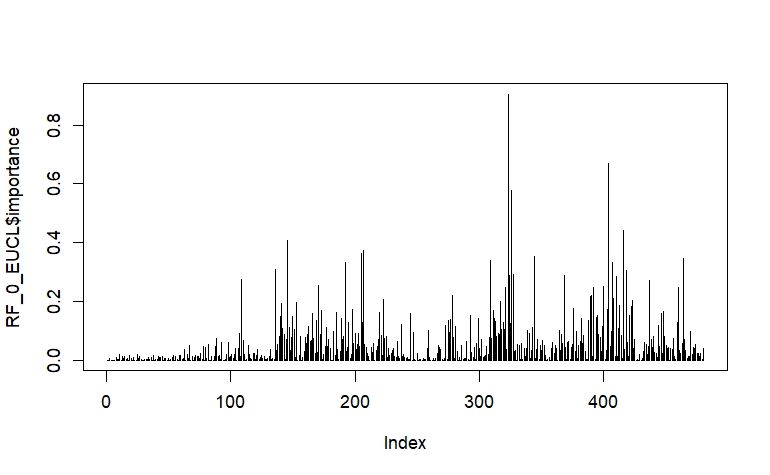
\includegraphics[width=0.45\textwidth]{img/01-5-eucl.png}}
    \subfigure[\textit{HR\_scaled}]{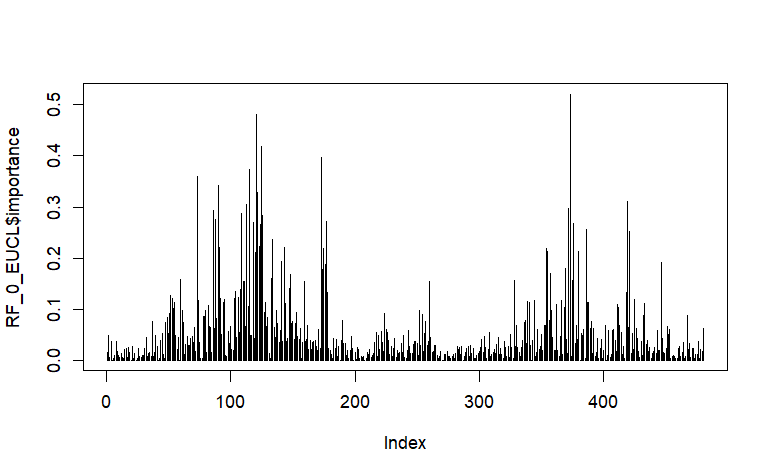
\includegraphics[width=0.45\textwidth]{img/02-5-eucl.png}}
    \subfigure[\textit{HR\_quantile}]{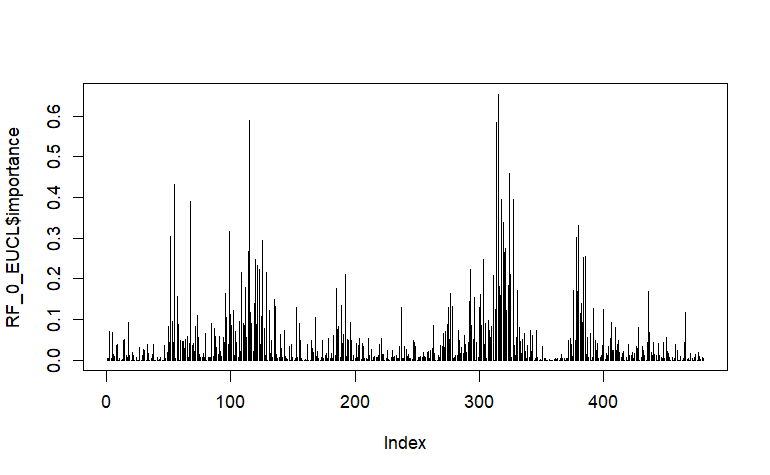
\includegraphics[width=0.5\textwidth]{img/03-5-eucl.png}}
    \caption{Importancia Raw Data de \textit{HR}, \textit{HR\_scaled} y \textit{HR\_quantile}}\label{fig:raw_data_imp_fc}
\end{figure}

\begin{figure}[ht]
    \centering
    \subfigure[\textit{SpO2}]{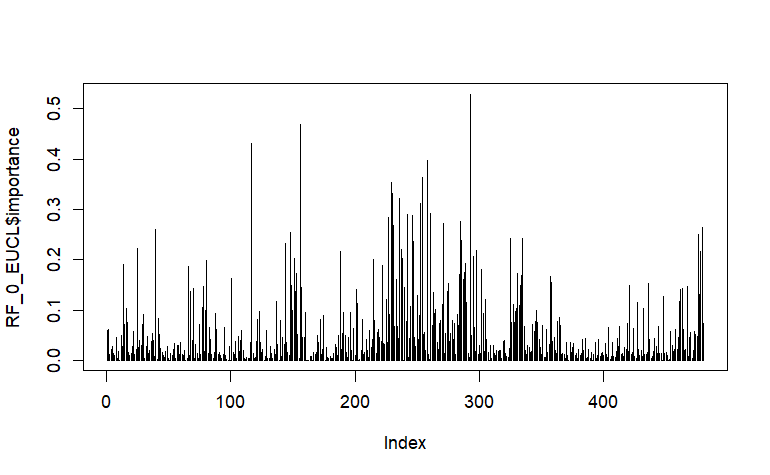
\includegraphics[width=0.5\textwidth]{img/04-5-eucl.png}}\hfill
    \subfigure[\textit{SpO2\_scaled}]{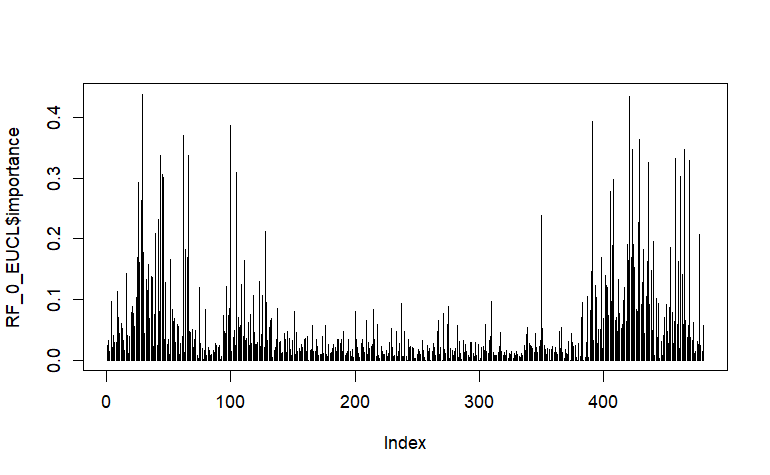
\includegraphics[width=0.5\textwidth]{img/05-5-eucl.png}}
    \caption{Importancia Raw Data de \textit{SpO2} y \textit{SpO2\_scaled}}\label{fig:raw_data_imp_spo2}
\end{figure}


\paragraph{Media de los valores de Raw Data en función de los clusters generados $k = 2$}

\begin{figure}[H]
    \centering
    \subfigure[\textit{HR}]{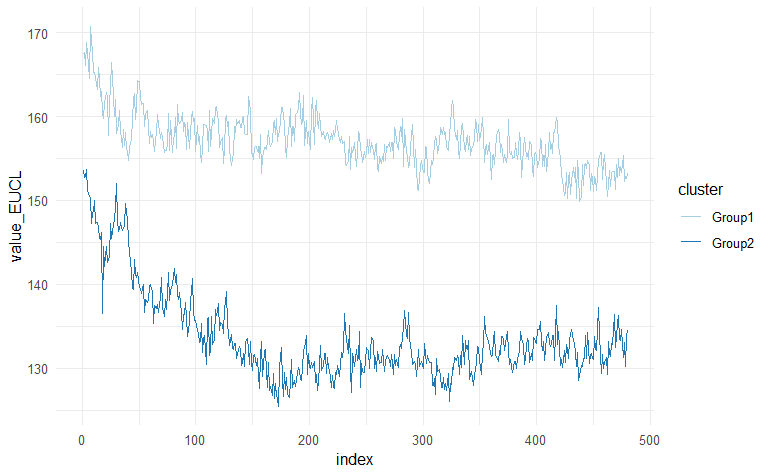
\includegraphics[width=0.45\textwidth]{img/01-6-eucl.png}}
    \subfigure[\textit{HR\_scaled}]{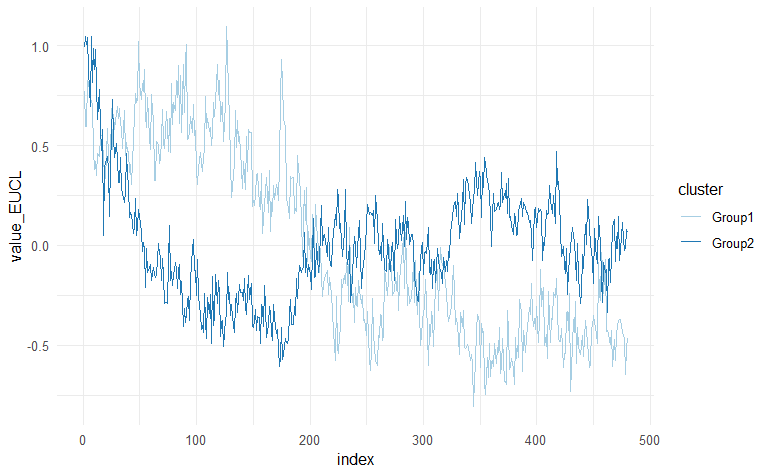
\includegraphics[width=0.45\textwidth]{img/02-6-eucl.png}}
    \subfigure[\textit{HR\_quantile}]{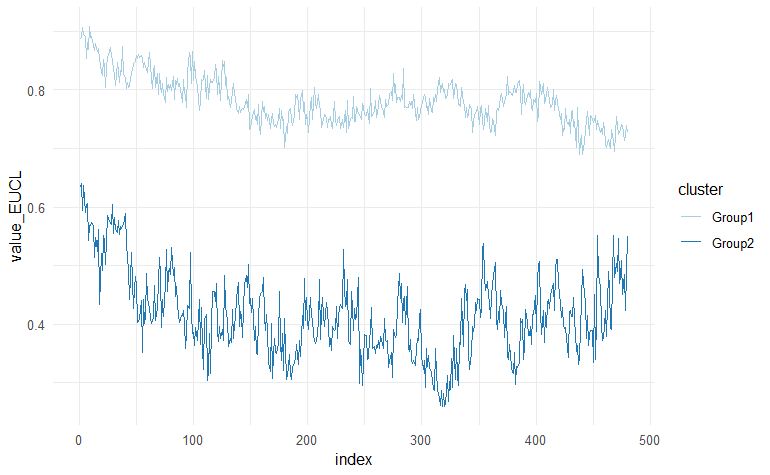
\includegraphics[width=0.5\textwidth]{img/03-6-eucl.png}}
    \caption{Valores de Raw Data por cluster k = 2 de \textit{HR}, \textit{HR\_scaled} y \textit{HR\_quantile}}\label{fig:raw_data_cls_fc}
\end{figure}

\begin{figure}[ht]
    \centering
    \subfigure[\textit{SpO2}]{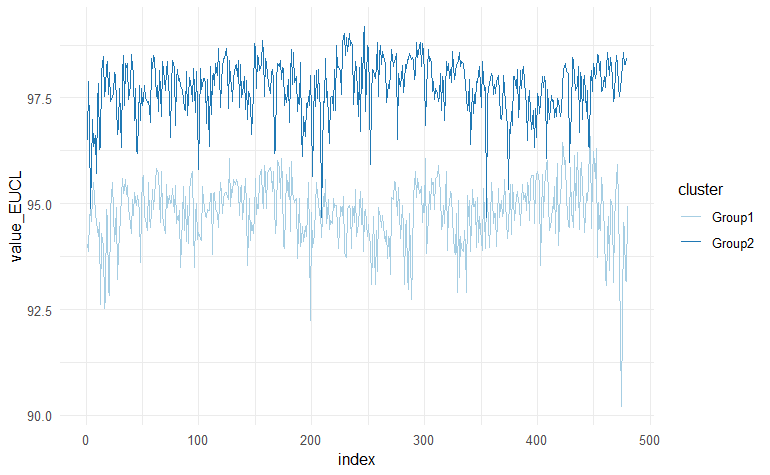
\includegraphics[width=0.5\textwidth]{img/04-6-eucl.png}}\hfill
    \subfigure[\textit{SpO2\_scaled}]{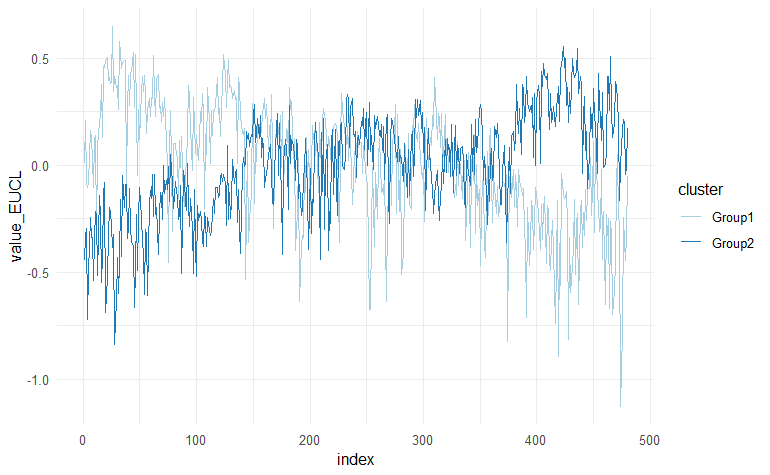
\includegraphics[width=0.5\textwidth]{img/05-6-eucl.png}}
    \caption{Valores de Raw Data por cluster k = 2 de \textit{SpO2} y \textit{SpO2\_scaled}}\label{fig:raw_data_cls_spo2}
\end{figure}


\newpage
\subsubsection{FAC}

\paragraph{Dendrograma de los clústeres obtenidos para FAC}

\begin{figure}[H]
    \centering
    
    \subfigure[\textit{HR}]{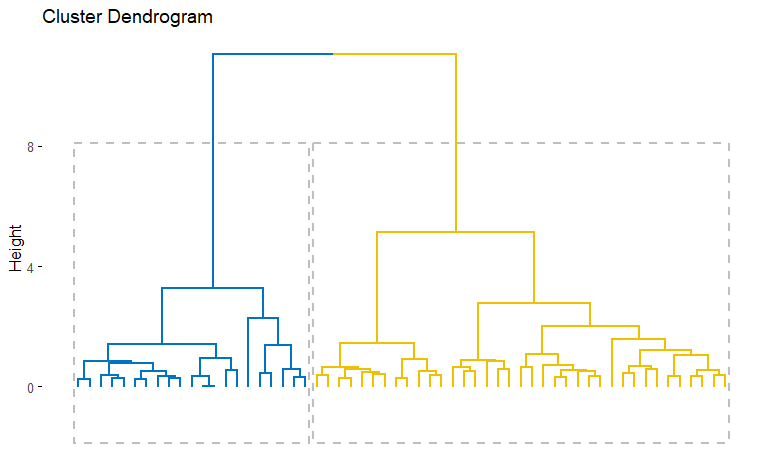
\includegraphics[width=0.45\textwidth]{img/01-1-acf.png}}
    \subfigure[\textit{HR\_scaled}]{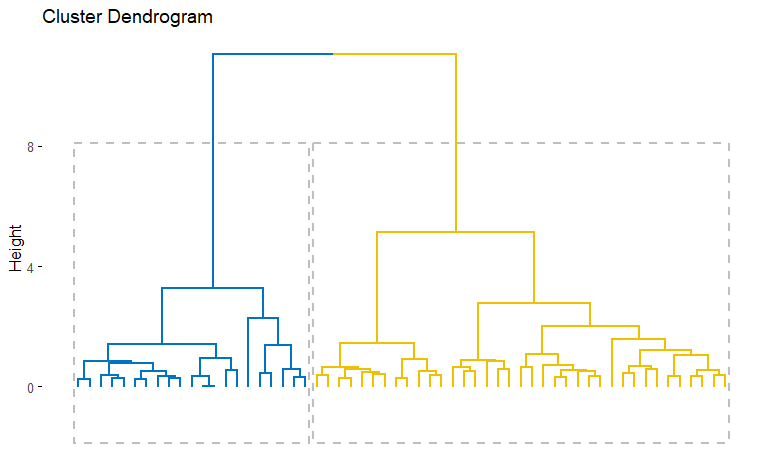
\includegraphics[width=0.45\textwidth]{img/02-1-acf.png}}
    \subfigure[\textit{HR\_quantile}]{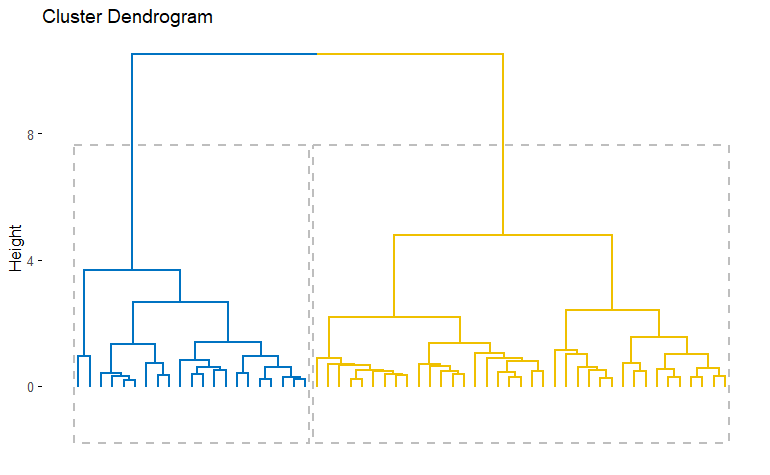
\includegraphics[width=0.5\textwidth]{img/03-1-acf.png}}
    \caption{Dendogramas usando FAC de \textit{HR}, \textit{HR\_scaled} y \textit{HR\_quantile}}
    \label{fig:acf_den_fc}
\end{figure}

\begin{figure}[ht]
    \centering
    \subfigure[\textit{SpO2}]{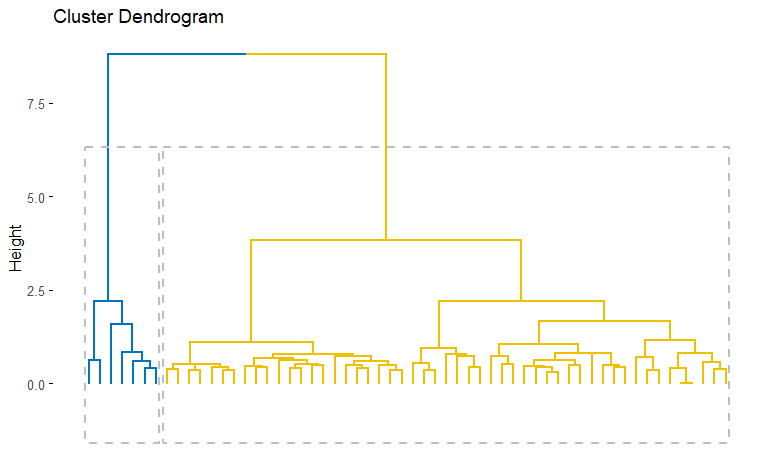
\includegraphics[width=0.5\textwidth]{img/04-1-acf.png}}\hfill
    \subfigure[\textit{SpO2\_scaled}]{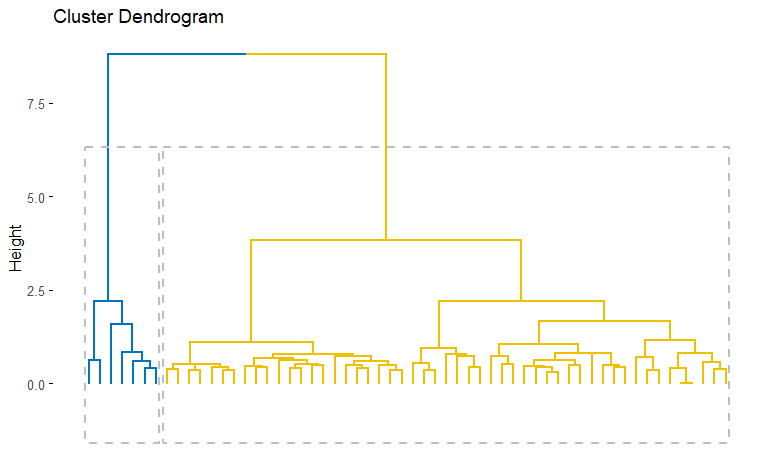
\includegraphics[width=0.5\textwidth]{img/05-1-acf.png}}
    \caption{Dendogramas usando FAC de \textit{SpO2} y \textit{SpO2\_scaled}}\label{fig:acf_den_spo2}
\end{figure}

\paragraph{Distribución de los clústeres obtenidos en función de las dos primeras componentes principales para FAC}

\begin{figure}[H]
    \centering
    \subfigure[\textit{HR}]{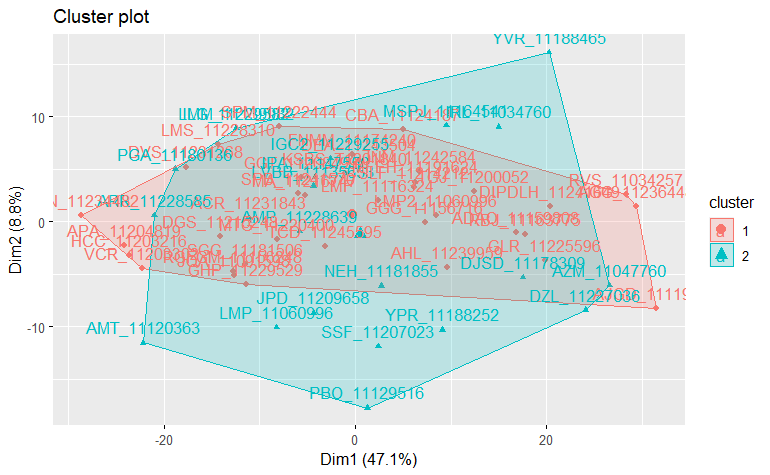
\includegraphics[width=0.45\textwidth]{img/01-2-acf.png}}
    \subfigure[\textit{HR\_scaled}]{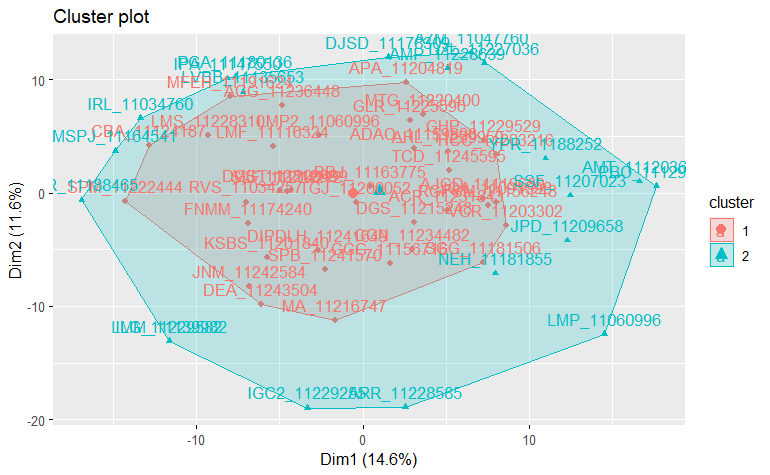
\includegraphics[width=0.45\textwidth]{img/02-2-acf.png}}
    \subfigure[\textit{HR\_quantile}]{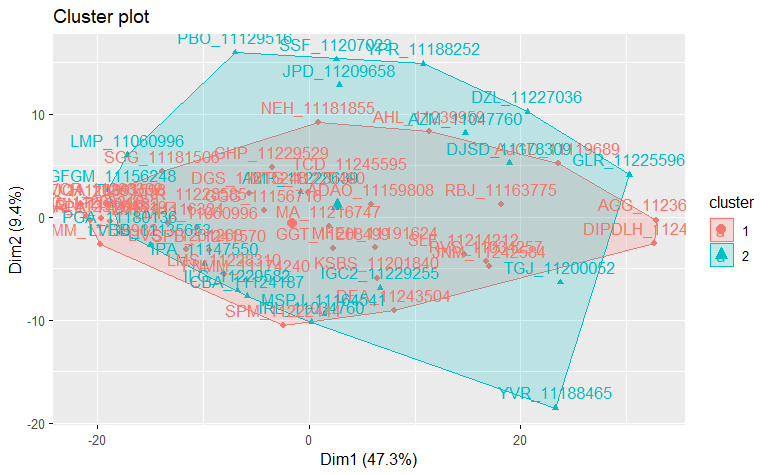
\includegraphics[width=0.5\textwidth]{img/03-2-acf.png}}
    \caption{Cluster Plot usando FAC de \textit{HR}, \textit{HR\_scaled} y \textit{HR\_quantile}}
    \label{fig:acf_pc_fc}
\end{figure}

\begin{figure}[H]
    \centering
    \subfigure[\textit{SpO2}]{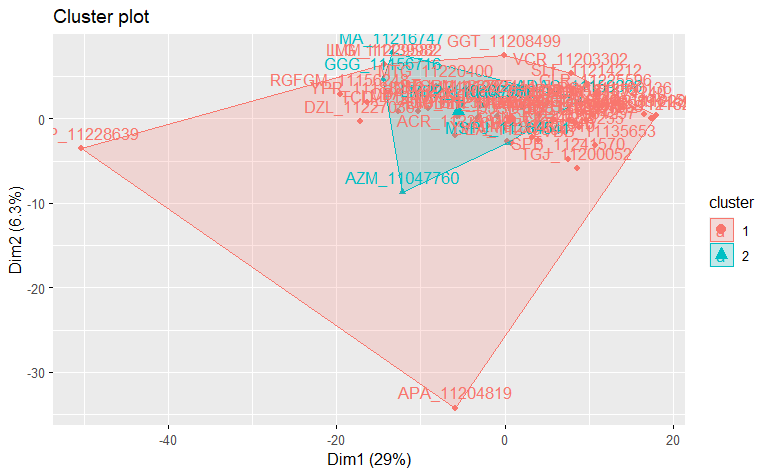
\includegraphics[width=0.5\textwidth]{img/04-2-acf.png}}\hfill
    \subfigure[\textit{SpO2\_scaled}]{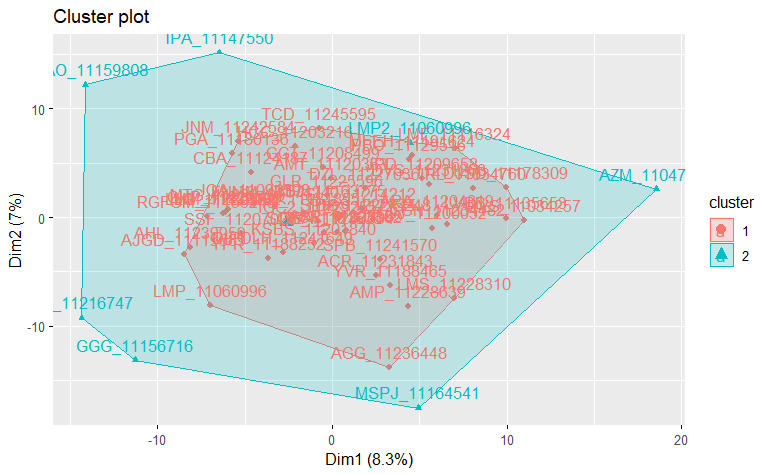
\includegraphics[width=0.5\textwidth]{img/05-2-acf.png}}
    \caption{Cluster Plot usando FAC de \textit{SpO2} y \textit{SpO2\_scaled}}\label{fig:acf_pc_spo2}
\end{figure}


\paragraph{Puntuación de Silhouette de los clústeres obtenidos para FAC}

\begin{figure}[H]
    \centering
    \subfigure[\textit{HR}]{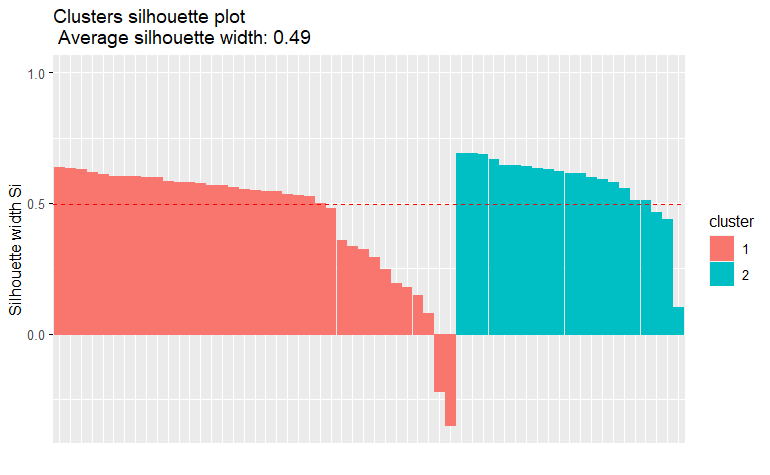
\includegraphics[width=0.45\textwidth]{img/01-3-acf.png}}
    \subfigure[\textit{HR\_scaled}]{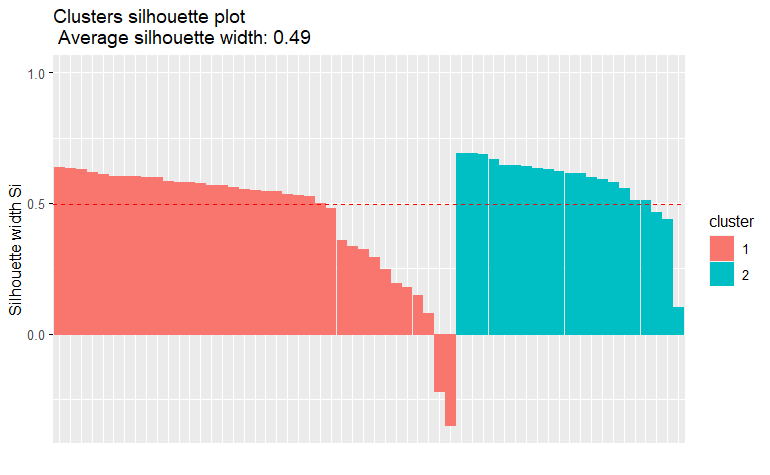
\includegraphics[width=0.45\textwidth]{img/02-3-acf.png}}
    \subfigure[\textit{HR\_quantile}]{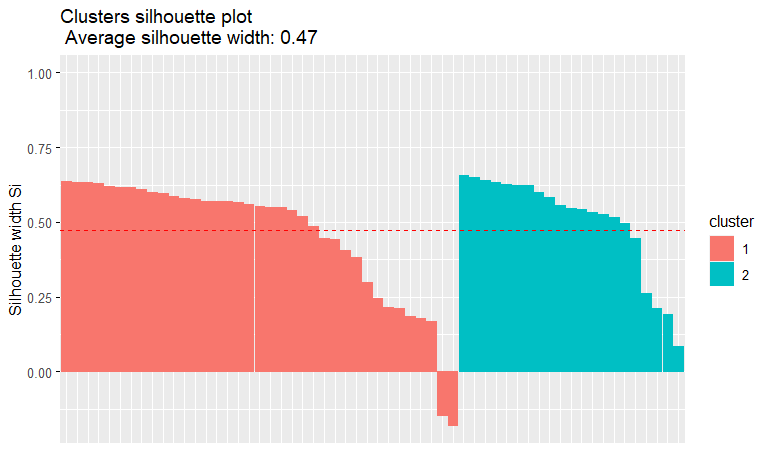
\includegraphics[width=0.5\textwidth]{img/03-3-acf.png}}
    \caption{Silhouette Plot usando FAC de \textit{HR}, \textit{HR\_scaled} y \textit{HR\_quantile}}\label{fig:acf_si_fc}
\end{figure}

\begin{figure}[ht]
    \centering
    \subfigure[\textit{SpO2}]{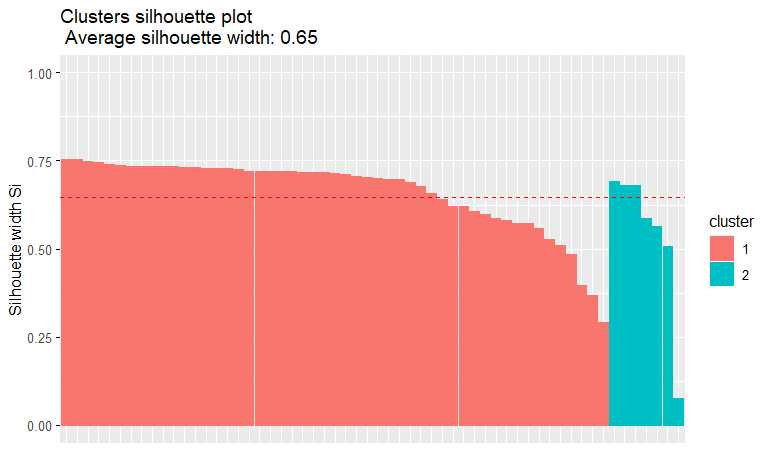
\includegraphics[width=0.5\textwidth]{img/04-3-acf.png}}\hfill
    \subfigure[\textit{SpO2\_scaled}]{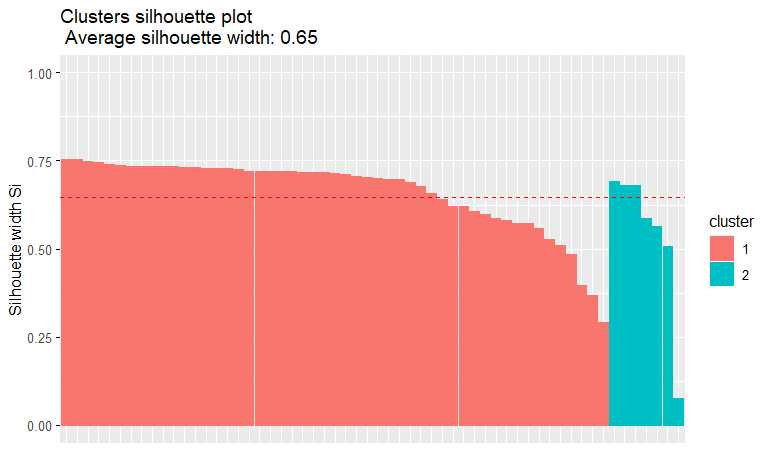
\includegraphics[width=0.5\textwidth]{img/05-3-acf.png}}
    \caption{Silhouette Plot usando FAC de \textit{SpO2} y \textit{SpO2\_scaled}}\label{fig:acf_si_spo2}
\end{figure}

\paragraph{Dendograma dividido en dos clústeres según los pacientes que han experimentado OAF para FAC}

\begin{figure}[H]
    \centering
    \subfigure[\textit{HR}]{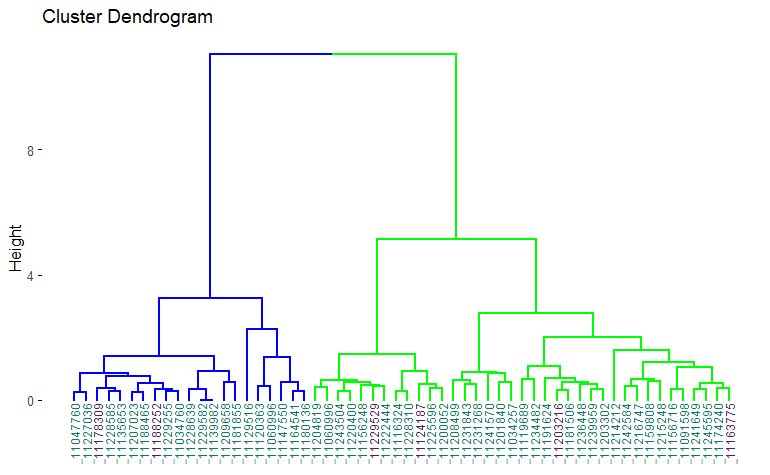
\includegraphics[width=0.45\textwidth]{img/01-4-acf.png}}
    \subfigure[\textit{HR\_scaled}]{\includegraphics[width=0.45\textwidth]{img/02-4-acf.png}}
    \subfigure[\textit{HR\_quantile}]{\includegraphics[width=0.5\textwidth]{img/03-4-acf.png}}
    \caption{Dendograma Plot k = 2 usando FAC de \textit{HR}, \textit{HR\_scaled} y \textit{HR\_quantile}}\label{fig:acf_ctg_fc}
\end{figure}

\begin{figure}[ht]
    \centering
    \subfigure[\textit{SpO2}]{\includegraphics[width=0.5\textwidth]{img/04-4-acf.png}}\hfill
    \subfigure[\textit{SpO2\_scaled}]{\includegraphics[width=0.5\textwidth]{img/05-4-acf.png}}
    \caption{Dendograma Plot k = 2 usando FAC de \textit{SpO2} y \textit{SpO2\_scaled}}\label{fig:acf_ctg_spo2}
\end{figure}

\paragraph{Clasificación mediente Random Forest de los clústeres generados con los datos de Peridiograma según las variables \textit{Cuantitativas} y \textit{Cualitativas} de la Tabla~\ref{tabla:variables_estudio_final} para FAC}

\begin{figure}[H]
    \centering
    \begin{lstlisting}[frame=single, basicstyle=\small\ttfamily]
        randomForest(formula = CLUSTER ~ ., data = newSMOTE_ACF) 
               Type of random forest: classification
                     Number of trees: 500
No. of variables tried at each split: 5

        OOB estimate of  error rate: 48.28%
Confusion matrix:
   1  2 class.error
1 26 11   0.2972973
2 17  4   0.8095238
    \end{lstlisting}
    \caption{Resultado de Random Forest usando FAC para \textit{HR} utilizando variables \textit{Cuantitativas} y \textit{Cualitativas} de la Tabla~\ref{tabla:variables_estudio_final} y clasificación de clusters k = 2}\label{fig:random_forest_acf_result_1}
\end{figure}
\begin{figure}[H]
    \centering
    \begin{lstlisting}[frame=single, basicstyle=\small\ttfamily]
        randomForest(formula = CLUSTER ~ ., data = newSMOTE_ACF) 
               Type of random forest: classification
                     Number of trees: 500
No. of variables tried at each split: 5

        OOB estimate of  error rate: 48.28%
Confusion matrix:
   1  2 class.error
1 26 11   0.2972973
2 17  4   0.8095238
    \end{lstlisting}
    \caption{Resultado de Random Forest usando FAC para \textit{HR\_scaled} utilizando variables \textit{Cuantitativas} y \textit{Cualitativas} de la Tabla~\ref{tabla:variables_estudio_final} y clasificación de clusters k = 2}
    \label{fig:random_forest_acf_result_2}
\end{figure}

\begin{figure}[H]
    \centering
    \begin{lstlisting}[frame=single, basicstyle=\small\ttfamily]
        randomForest(formula = CLUSTER ~ ., data = newMWMOTE_ACF) 
               Type of random forest: classification
                     Number of trees: 500
No. of variables tried at each split: 5

        OOB estimate of  error rate: 32.76%
Confusion matrix:
   1 2 class.error
1 30 7   0.1891892
2 12 9   0.5714286
    \end{lstlisting}
    \caption{Resultado de Random Forest usando FAC para \textit{HR\_quantile} utilizando variables \textit{Cuantitativas} y \textit{Cualitativas} de la Tabla~\ref{tabla:variables_estudio_final} y clasificación de clusters k = 2}
    \label{fig:random_forest_acf_result_3}
\end{figure}

\begin{figure}[H]
    \centering
    \begin{lstlisting}[frame=single, basicstyle=\small\ttfamily]
        randomForest(formula = CLUSTER ~ ., data = newSMOTE_ACF) 
               Type of random forest: classification
                     Number of trees: 500
No. of variables tried at each split: 5

        OOB estimate of  error rate: 5.26%
Confusion matrix:
   1  2 class.error
1 49  2  0.03921569
2  3 41  0.06818182
    \end{lstlisting}
    \caption{Resultado de Random Forest usando FAC para \textit{SpO2} utilizando variables \textit{Cuantitativas} y \textit{Cualitativas} de la Tabla~\ref{tabla:variables_estudio_final} y clasificación de clusters k = 2}\label{fig:random_forest_acf_result_4}
\end{figure}
\begin{figure}[H]
    \centering
    \begin{lstlisting}[frame=single, basicstyle=\small\ttfamily]
        randomForest(formula = CLUSTER ~ ., data = newSMOTE_ACF) 
               Type of random forest: classification
                     Number of trees: 500
No. of variables tried at each split: 5

        OOB estimate of  error rate: 5.26%
Confusion matrix:
   1  2 class.error
1 49  2  0.03921569
2  3 41  0.06818182
    \end{lstlisting}
    \caption{Resultado de Random Forest usando FAC para \textit{SpO2\_scaled} utilizando variables \textit{Cuantitativas} y \textit{Cualitativas} de la Tabla~\ref{tabla:variables_estudio_final} y clasificación de clusters k = 2}
    \label{fig:random_forest_acf_result_5}
\end{figure}

\paragraph{Mean Decrease Accuracy de las 5 primeras variables descriptivas utilizadas en Random Forest para FAC}

\begin{table}[H]
    \centering
    \begin{tabular}{lr}
        \toprule
        \textbf{Variable} & \textbf{Mean Decrease Accuracy} \\
        \midrule
        EDAD & 2.6328715 \\
        SCORE\_WOOD\_DOWNES\_INGRESO & 2.5338316 \\
        PESO & 2.3967813 \\
        SCORE\_CRUCES\_INGRESO & 2.3630299 \\
        FR\_0\_8h & 1.7007907 \\
        \bottomrule
    \end{tabular}
    \caption{Mean Decrease Accuracy usando FAC \textit{HR}}
\end{table}

\begin{table}[H]
    \centering
    \begin{tabular}{lr}
        \toprule
        \textbf{Variable} & \textbf{Mean Decrease Accuracy} \\
        \midrule
        EDAD & 2.6328715 \\
        SCORE\_WOOD\_DOWNES\_INGRESO & 2.5338316 \\
        PESO & 2.3967813 \\
        SCORE\_CRUCES\_INGRESO & 2.3630299 \\
        FR\_0\_8h & 1.7007907 \\
        \bottomrule
    \end{tabular}
    \caption{Mean Decrease Accuracy usando FAC \textit{HR\_scaled}}
\end{table}

\begin{table}[H]
    \centering
    \begin{tabular}{lr}
        \toprule
        \textbf{Variable} & \textbf{Mean Decrease Accuracy} \\
        \midrule
        SCORE\_WOOD\_DOWNES\_INGRESO & 3.1336476 \\
        PESO & 3.1080877 \\
        EDAD & 2.5533093 \\
        SCORE\_CRUCES\_INGRESO & 2.3892629 \\
        FR\_0\_8h & 1.7130177 \\
        \bottomrule
    \end{tabular}
    \caption{Mean Decrease Accuracy usando FAC \textit{HR\_quantile}} 
\end{table}

\begin{table}[H]
    \centering
    \begin{tabular}{lr}
        \toprule
        \textbf{Variable} & \textbf{Mean Decrease Accuracy} \\
        \midrule
        SCORE\_CRUCES\_INGRESO & 6.6714244 \\
        SAPI\_0\_8h & 6.2990402 \\
        SCORE\_WOOD\_DOWNES\_INGRESO & 5.7922765 \\
        ENFERMEDAD\_BASE & 4.3830928 \\
        EDAD & 2.9415274 \\
        \bottomrule
    \end{tabular}
    \caption{Mean Decrease Accuracy usando FAC \textit{SpO2}}
\end{table}

\begin{table}[H]
    \centering
    \begin{tabular}{lr}
        \toprule
        \textbf{Variable} & \textbf{Mean Decrease Accuracy} \\
        \midrule
        SAPI\_0\_8h & 7.3979738 \\
        SCORE\_CRUCES\_INGRESO & 6.7882670 \\
        SCORE\_WOOD\_DOWNES\_INGRESO & 5.2945505 \\
        ENFERMEDAD\_BASE & 3.1331112 \\
        DIAS\_GN & 3.0845580 \\
        \bottomrule
    \end{tabular}
    \caption{Mean Decrease Accuracy usando FAC \textit{SpO2\_scaled}}
\end{table}


\paragraph{Clasificación mediente Random Forest de los clústeres según FAC utilizada para genear los mismos} 

\begin{figure}[H]
    \centering
    \begin{lstlisting}[frame=single, basicstyle=\small\ttfamily]
        randomForest(formula = CLUSTER ~ ., data = data_frame_merge_ACF) 
               Type of random forest: classification
                     Number of trees: 500
No. of variables tried at each split: 7

        OOB estimate of  error rate: 1.72%
Confusion matrix:
   1  2 class.error
1 37  0  0.00000000
2  1 20  0.04761905
    \end{lstlisting}
    \caption{Resultado de Random Forest usando FAC para \textit{HR} utilizando FAC y clasificación de clusters k = 2}\label{fig:random_forest_acf_result_RF_1}
\end{figure}
\begin{figure}[H]
    \centering
    \begin{lstlisting}[frame=single, basicstyle=\small\ttfamily]
        randomForest(formula = CLUSTER ~ ., data = data_frame_merge_ACF) 
               Type of random forest: classification
                     Number of trees: 500
No. of variables tried at each split: 7

        OOB estimate of  error rate: 1.72%
Confusion matrix:
   1  2 class.error
1 37  0  0.00000000
2  1 20  0.04761905
    \end{lstlisting}
    \caption{Resultado de Random Forest usando FAC para \textit{HR\_scaled} utilizando FAC y clasificación de clusters k = 2}
    \label{fig:random_forest_acf_result_RF_2}
\end{figure}

\begin{figure}[H]
    \centering
    \begin{lstlisting}[frame=single, basicstyle=\small\ttfamily]
        randomForest(formula = CLUSTER ~ ., data = data_frame_merge_ACF) 
               Type of random forest: classification
                     Number of trees: 500
No. of variables tried at each split: 7

        OOB estimate of  error rate: 3.45%
Confusion matrix:
   1  2 class.error
1 36  1  0.02702703
2  1 20  0.04761905
    \end{lstlisting}
    \caption{Resultado de Random Forest usando FAC para \textit{HR\_quantile} utilizando FAC y clasificación de clusters k = 2}
    \label{fig:random_forest_acf_result_RF_3}
\end{figure}

\begin{figure}[H]
    \centering
    \begin{lstlisting}[frame=single, basicstyle=\small\ttfamily]
        randomForest(formula = CLUSTER ~ ., data = data_frame_merge_ACF) 
               Type of random forest: classification
                     Number of trees: 500
No. of variables tried at each split: 7

        OOB estimate of  error rate: 1.72%
Confusion matrix:
   1 2 class.error
1 51 0   0.0000000
2  1 6   0.1428571
    \end{lstlisting}
    \caption{Resultado de Random Forest usando FAC para \textit{SpO2} utilizando FAC y clasificación de clusters k = 2}\label{fig:random_forest_acf_result_RF_4}
\end{figure}
\begin{figure}[H]
    \centering
    \begin{lstlisting}[frame=single, basicstyle=\small\ttfamily]
        randomForest(formula = CLUSTER ~ ., data = data_frame_merge_ACF) 
               Type of random forest: classification
                     Number of trees: 500
No. of variables tried at each split: 7

        OOB estimate of  error rate: 1.72%
Confusion matrix:
   1 2 class.error
1 51 0   0.0000000
2  1 6   0.1428571
    \end{lstlisting}
    \caption{Resultado de Random Forest usando FAC para \textit{SpO2\_scaled} utilizando FAC y clasificación de clusters k = 2}
    \label{fig:random_forest_acf_result_RF_5}
\end{figure}

\paragraph{Distribución de la Importancia de FAC}

\begin{figure}[H]
    \centering
    \subfigure[\textit{HR}]{\includegraphics[width=0.45\textwidth]{img/01-5-acf.png}}
    \subfigure[\textit{HR\_scaled}]{\includegraphics[width=0.45\textwidth]{img/02-5-acf.png}}
    \subfigure[\textit{HR\_quantile}]{\includegraphics[width=0.5\textwidth]{img/03-5-acf.png}}
    \caption{Importancia FAC de \textit{HR}, \textit{HR\_scaled} y \textit{HR\_quantile}}\label{fig:acf_imp_fc}
\end{figure}

\begin{figure}[ht]
    \centering
    \subfigure[\textit{SpO2}]{\includegraphics[width=0.5\textwidth]{img/04-5-acf.png}}\hfill
    \subfigure[\textit{SpO2\_scaled}]{\includegraphics[width=0.5\textwidth]{img/05-5-acf.png}}
    \caption{Importancia FAC de \textit{SpO2} y \textit{SpO2\_scaled}}\label{fig:acf_imp_spo2}
\end{figure}


\paragraph{Media de los valores de FAC en función de los clusters generados $k = 2$}

\begin{figure}[H]
    \centering
    \subfigure[\textit{HR}]{\includegraphics[width=0.45\textwidth]{img/01-6-acf.png}}
    \subfigure[\textit{HR\_scaled}]{\includegraphics[width=0.45\textwidth]{img/02-6-acf.png}}
    \subfigure[\textit{HR\_quantile}]{\includegraphics[width=0.5\textwidth]{img/03-6-acf.png}}
    \caption{Valores de FAC por cluster k = 2 de \textit{HR}, \textit{HR\_scaled} y \textit{HR\_quantile}}\label{fig:acf_cls_fc}
\end{figure}

\begin{figure}[ht]
    \centering
    \subfigure[\textit{SpO2}]{\includegraphics[width=0.5\textwidth]{img/04-6-acf.png}}\hfill
    \subfigure[\textit{SpO2\_scaled}]{\includegraphics[width=0.5\textwidth]{img/05-6-acf.png}}
    \caption{Valores de FAC por cluster k = 2 de \textit{SpO2} y \textit{SpO2\_scaled}}\label{fig:acf_cls_spo2}
\end{figure}



\newpage
\subsubsection{Peridiograma}

\paragraph{Dendrograma de los clústeres obtenidos para Peridiograma}

\begin{figure}[H]
    \centering
    
    \subfigure[\textit{HR}]{\includegraphics[width=0.45\textwidth]{img/01-1-per.png}}
    \subfigure[\textit{HR\_scaled}]{\includegraphics[width=0.45\textwidth]{img/02-1-per.png}}
    \subfigure[\textit{HR\_quantile}]{\includegraphics[width=0.5\textwidth]{img/03-1-per.png}}
    \caption{Dendogramas usando Peridiograma de \textit{HR}, \textit{HR\_scaled} y \textit{HR\_quantile}}
    \label{fig:per_den_fc}
\end{figure}

\begin{figure}[ht]
    \centering
    \subfigure[\textit{SpO2}]{\includegraphics[width=0.5\textwidth]{img/04-1-per.png}}\hfill
    \subfigure[\textit{SpO2\_scaled}]{\includegraphics[width=0.5\textwidth]{img/05-1-per.png}}
    \caption{Dendogramas usando Peridiograma de \textit{SpO2} y \textit{SpO2\_scaled}}\label{fig:per_den_spo2}
\end{figure}

\paragraph{Distribución de los clústeres obtenidos en función de las dos primeras componentes principales}

\begin{figure}[H]
    \centering
    \subfigure[\textit{HR}]{\includegraphics[width=0.45\textwidth]{img/01-2-per.png}}
    \subfigure[\textit{HR\_scaled}]{\includegraphics[width=0.45\textwidth]{img/02-2-per.png}}
    \subfigure[\textit{HR\_quantile}]{\includegraphics[width=0.5\textwidth]{img/03-2-per.png}}
    \caption{Cluster Plot usando Peridiograma de \textit{HR}, \textit{HR\_scaled} y \textit{HR\_quantile}}
    \label{fig:per_pc_fc}
\end{figure}

\begin{figure}[ht]
    \centering
    \subfigure[\textit{SpO2}]{\includegraphics[width=0.5\textwidth]{img/04-2-per.png}}\hfill
    \subfigure[\textit{SpO2\_scaled}]{\includegraphics[width=0.5\textwidth]{img/05-2-per.png}}
    \caption{Cluster Plot usando Peridiograma de \textit{SpO2} y \textit{SpO2\_scaled}}\label{fig:per_pc_spo2}
\end{figure}


\paragraph{Puntuación de Silhouette de los clústeres obtenidos}

\begin{figure}[H]
    \centering
    \subfigure[\textit{HR}]{\includegraphics[width=0.45\textwidth]{img/01-3-per.png}}
    \subfigure[\textit{HR\_scaled}]{\includegraphics[width=0.45\textwidth]{img/02-3-per.png}}
    \subfigure[\textit{HR\_quantile}]{\includegraphics[width=0.5\textwidth]{img/03-3-per.png}}
    \caption{Silhouette Plot usando Peridiograma de \textit{HR}, \textit{HR\_scaled} y \textit{HR\_quantile}}\label{fig:per_si_fc}
\end{figure}

\begin{figure}[ht]
    \centering
    \subfigure[\textit{SpO2}]{\includegraphics[width=0.5\textwidth]{img/04-3-per.png}}\hfill
    \subfigure[\textit{SpO2\_scaled}]{\includegraphics[width=0.5\textwidth]{img/05-3-per.png}}
    \caption{Silhouette Plot usando Peridiograma de \textit{SpO2} y \textit{SpO2\_scaled}}\label{fig:per_si_spo2}
\end{figure}

\paragraph{Dendograma dividido en dos clústeres según los pacientes que han experimentado OAF para Peridiograma}

\begin{figure}[H]
    \centering
    \subfigure[\textit{HR}]{\includegraphics[width=0.45\textwidth]{img/01-4-per.png}}
    \subfigure[\textit{HR\_scaled}]{\includegraphics[width=0.45\textwidth]{img/02-4-per.png}}
    \subfigure[\textit{HR\_quantile}]{\includegraphics[width=0.5\textwidth]{img/03-4-per.png}}
    \caption{Dendograma Plot k = 2 usando Peridiograma de \textit{HR}, \textit{HR\_scaled} y \textit{HR\_quantile}}\label{fig:per_ctg_fc}
\end{figure}

\begin{figure}[ht]
    \centering
    \subfigure[\textit{SpO2}]{\includegraphics[width=0.5\textwidth]{img/04-4-per.png}}\hfill
    \subfigure[\textit{SpO2\_scaled}]{\includegraphics[width=0.5\textwidth]{img/05-4-per.png}}
    \caption{Dendograma Plot k = 2 usando Peridiograma de \textit{SpO2} y \textit{SpO2\_scaled}}\label{fig:per_ctg_spo2}
\end{figure}

\paragraph{Clasificación mediente Random Forest de los clústeres según las variables \textit{Cuantitativas} y \textit{Cualitativas} de la Tabla~\ref{tabla:variables_estudio_final} para Peridiograma}

\begin{figure}[H]
    \centering
    \begin{lstlisting}[frame=single, basicstyle=\small\ttfamily]
        randomForest(formula = CLUSTER ~ ., data = newSMOTE_PER) 
               Type of random forest: classification
                     Number of trees: 500
No. of variables tried at each split: 5

        OOB estimate of  error rate: 6.45%
Confusion matrix:
   1  2 class.error
1 49  1   0.0200000
2  5 38   0.1162791
    \end{lstlisting}
    \caption{Resultado de Random Forest usando Peridiograma para \textit{HR} utilizando variables \textit{Cuantitativas} y \textit{Cualitativas} de la Tabla~\ref{tabla:variables_estudio_final} y clasificación de clusters k = 2}\label{fig:random_forest_per_result_1}
\end{figure}
\begin{figure}[H]
    \centering
    \begin{lstlisting}[frame=single, basicstyle=\small\ttfamily]
        randomForest(formula = CLUSTER ~ ., data = newSMOTE_PER) 
               Type of random forest: classification
                     Number of trees: 500
No. of variables tried at each split: 5

        OOB estimate of  error rate: 37.93%
Confusion matrix:
   1 2 class.error
1 28 8   0.2222222
2 14 8   0.6363636
    \end{lstlisting}
    \caption{Resultado de Random Forest usando Peridiograma para \textit{HR\_scaled} utilizando variables \textit{Cuantitativas} y \textit{Cualitativas} de la Tabla~\ref{tabla:variables_estudio_final} y clasificación de clusters k = 2}
    \label{fig:random_forest_per_result_2}
\end{figure}

\begin{figure}[H]
    \centering
    \begin{lstlisting}[frame=single, basicstyle=\small\ttfamily]
        randomForest(formula = CLUSTER ~ ., data = newMWMOTE_PER) 
               Type of random forest: classification
                     Number of trees: 500
No. of variables tried at each split: 5

        OOB estimate of  error rate: 4.3%
Confusion matrix:
   1  2 class.error
1 47  3  0.06000000
2  1 42  0.02325581
    \end{lstlisting}
    \caption{Resultado de Random Forest usando Peridiograma para \textit{HR\_quantile} utilizando variables \textit{Cuantitativas} y \textit{Cualitativas} de la Tabla~\ref{tabla:variables_estudio_final} y clasificación de clusters k = 2}
    \label{fig:random_forest_per_result_3}
\end{figure}

\begin{figure}[H]
    \centering
    \begin{lstlisting}[frame=single, basicstyle=\small\ttfamily]
        randomForest(formula = CLUSTER ~ ., data = newSMOTE_PER) 
               Type of random forest: classification
                     Number of trees: 500
No. of variables tried at each split: 5

        OOB estimate of  error rate: 7.53%
Confusion matrix:
   1  2 class.error
1 48  2   0.0400000
2  5 38   0.1162791
    \end{lstlisting}
    \caption{Resultado de Random Forest usando Peridiograma para \textit{SpO2} utilizando variables \textit{Cuantitativas} y \textit{Cualitativas} de la Tabla~\ref{tabla:variables_estudio_final} y clasificación de clusters k = 2}\label{fig:random_forest_per_result_4}
\end{figure}
\begin{figure}[H]
    \centering
    \begin{lstlisting}[frame=single, basicstyle=\small\ttfamily]
        randomForest(formula = CLUSTER ~ ., data = newSMOTE_PER) 
               Type of random forest: classification
                     Number of trees: 500
No. of variables tried at each split: 5

        OOB estimate of  error rate: 14.29%
Confusion matrix:
   1  2 class.error
1 41  4  0.08888889
2  8 31  0.20512821
    \end{lstlisting}
    \caption{Resultado de Random Forest usando Peridiograma para \textit{SpO2\_scaled} utilizando variables \textit{Cuantitativas} y \textit{Cualitativas} de la Tabla~\ref{tabla:variables_estudio_final} y clasificación de clusters k = 2}
    \label{fig:random_forest_per_result_5}
\end{figure}

\paragraph{Mean Decrease Accuracy de las 5 primeras variables descriptivas utilizadas en Random Forest para Peridiograma}

\begin{table}[H]
    \centering
    \begin{tabular}{lr}
        \toprule
        \textbf{Variable} & \textbf{Mean Decrease Accuracy} \\
        \midrule
        SCORE\_CRUCES\_INGRESO & 8.9852612 \\
        SCORE\_WOOD\_DOWNES\_INGRESO & 5.2582849 \\
        RADIOGRAFIA & 5.1448815 \\
        SAPI\_0\_8h & 4.2663169 \\
        PESO & 2.6165359 \\
        \bottomrule
    \end{tabular}
    \caption{Mean Decrease Accuracy usando Peridiograma \textit{HR}}
\end{table}

\begin{table}[H]
    \centering
    \begin{tabular}{lr}
        \toprule
        \textbf{Variable} & \textbf{Mean Decrease Accuracy} \\
        \midrule
        PESO & 2.8009743 \\
        RADIOGRAFIA & 2.6058470 \\
        EDAD & 2.4925543 \\
        FR\_0\_8h & 2.4681832 \\
        SCORE\_WOOD\_DOWNES\_INGRESO & 2.0989243 \\
        \bottomrule
    \end{tabular}
    \caption{Mean Decrease Accuracy usando Peridiograma \textit{HR\_scaled}}
\end{table}

\begin{table}[H]
    \centering
    \begin{tabular}{lr}
        \toprule
        \textbf{Variable} & \textbf{Mean Decrease Accuracy} \\
        \midrule
        SCORE\_WOOD\_DOWNES\_INGRESO & 7.4074045 \\
        SCORE\_CRUCES\_INGRESO & 6.5504895 \\
        SAPI\_0\_8h & 4.0000376 \\
        DIAS\_O2\_TOTAL & 2.9619896 \\
        EDAD & 2.9220530 \\
        \bottomrule
    \end{tabular}
    \caption{Mean Decrease Accuracy usando Peridiograma \textit{HR\_quantile}} 
\end{table}

\begin{table}[H]
    \centering
    \begin{tabular}{lr}
        \toprule
        \textbf{Variable} & \textbf{Mean Decrease Accuracy} \\
        \midrule
        SCORE\_WOOD\_DOWNES\_INGRESO & 9.4039903 \\
        SCORE\_CRUCES\_INGRESO & 5.8936796 \\
        SAPI\_0\_8h & 2.9363664 \\
        ETIOLOGIA & 2.5904366 \\
        TABACO & 2.4803961 \\
        \bottomrule
    \end{tabular}
    \caption{Mean Decrease Accuracy usando Peridiograma \textit{SpO2}}
\end{table}

\begin{table}[H]
    \centering
    \begin{tabular}{lr}
        \toprule
        \textbf{Variable} & \textbf{Mean Decrease Accuracy} \\
        \midrule
        SAPI\_0\_8h & 5.9478329 \\
        EDAD & 4.8844865 \\
        PESO & 4.4966094 \\
        SCORE\_WOOD\_DOWNES\_INGRESO & 3.8820332 \\
        SCORE\_CRUCES\_INGRESO & 3.3041235 \\
        \bottomrule
    \end{tabular}
    \caption{Mean Decrease Accuracy usando Peridiograma \textit{SpO2\_scaled}}
\end{table}


\paragraph{Clasificación mediente Random Forest de los clústeres según Peridiograma utilizada para genear los mismos para Peridiograma} 

\begin{figure}[H]
    \centering
    \begin{lstlisting}[frame=single, basicstyle=\small\ttfamily]
        randomForest(formula = CLUSTER ~ ., data = data_frame_merge_PER) 
               Type of random forest: classification
                     Number of trees: 500
No. of variables tried at each split: 21

        OOB estimate of  error rate: 13.79%
Confusion matrix:
   1 2 class.error
1 50 0           0
2  8 0           1
    \end{lstlisting}
    \caption{Resultado de Random Forest usando Peridiograma para \textit{HR} utilizando Peridiograma y clasificación de clusters k = 2}\label{fig:random_forest_per_result_RF_1}
\end{figure}
\begin{figure}[H]
    \centering
    \begin{lstlisting}[frame=single, basicstyle=\small\ttfamily]
        randomForest(formula = CLUSTER ~ ., data = data_frame_merge_PER) 
               Type of random forest: classification
                     Number of trees: 500
No. of variables tried at each split: 21

        OOB estimate of  error rate: 13.79%
Confusion matrix:
   1  2 class.error
1 35  1  0.02777778
2  7 15  0.31818182
    \end{lstlisting}
    \caption{Resultado de Random Forest usando Peridiograma para \textit{HR\_scaled} utilizando Peridiograma y clasificación de clusters k = 2}
    \label{fig:random_forest_per_result_RF_2}
\end{figure}

\begin{figure}[H]
    \centering
    \begin{lstlisting}[frame=single, basicstyle=\small\ttfamily]
        randomForest(formula = CLUSTER ~ ., data = data_frame_merge_PER) 
               Type of random forest: classification
                     Number of trees: 500
No. of variables tried at each split: 21

        OOB estimate of  error rate: 13.79%
Confusion matrix:
   1 2 class.error
1 50 0           0
2  8 0           1
    \end{lstlisting}
    \caption{Resultado de Random Forest usando Peridiograma para \textit{HR\_quantile} utilizando Peridiograma y clasificación de clusters k = 2}
    \label{fig:random_forest_per_result_RF_3}
\end{figure}

\begin{figure}[H]
    \centering
    \begin{lstlisting}[frame=single, basicstyle=\small\ttfamily]
        randomForest(formula = CLUSTER ~ ., data = data_frame_merge_PER) 
               Type of random forest: classification
                     Number of trees: 500
No. of variables tried at each split: 21

        OOB estimate of  error rate: 8.62%
Confusion matrix:
   1 2 class.error
1 50 0       0.000
2  5 3       0.625
    \end{lstlisting}
    \caption{Resultado de Random Forest usando Peridiograma para \textit{SpO2} utilizando Peridiograma y clasificación de clusters k = 2}\label{fig:random_forest_per_result_RF_4}
\end{figure}
\begin{figure}[H]
    \centering
    \begin{lstlisting}[frame=single, basicstyle=\small\ttfamily]
        randomForest(formula = CLUSTER ~ ., data = data_frame_merge_PER) 
               Type of random forest: classification
                     Number of trees: 500
No. of variables tried at each split: 21

        OOB estimate of  error rate: 12.07%
Confusion matrix:
   1 2 class.error
1 45 0   0.0000000
2  7 6   0.5384615
    \end{lstlisting}
    \caption{Resultado de Random Forest usando Peridiograma para \textit{SpO2\_scaled} utilizando Peridiograma y clasificación de clusters k = 2}
    \label{fig:random_forest_per_result_RF_5}
\end{figure}

\paragraph{Distribución de la Importancia de Peridiograma}

\begin{figure}[H]
    \centering
    \subfigure[\textit{HR}]{\includegraphics[width=0.45\textwidth]{img/01-5-per.png}}
    \subfigure[\textit{HR\_scaled}]{\includegraphics[width=0.45\textwidth]{img/02-5-per.png}}
    \subfigure[\textit{HR\_quantile}]{\includegraphics[width=0.5\textwidth]{img/03-5-per.png}}
    \caption{Importancia Peridiograma de \textit{HR}, \textit{HR\_scaled} y \textit{HR\_quantile}}\label{fig:per_imp_fc}
\end{figure}

\begin{figure}[ht]
    \centering
    \subfigure[\textit{SpO2}]{\includegraphics[width=0.5\textwidth]{img/04-5-per.png}}\hfill
    \subfigure[\textit{SpO2\_scaled}]{\includegraphics[width=0.5\textwidth]{img/05-5-per.png}}
    \caption{Importancia Peridiograma de \textit{SpO2} y \textit{SpO2\_scaled}}\label{fig:per_imp_spo2}
\end{figure}


\paragraph{Media de los valores de Peridiograma en función de los clusters generados $k = 2$}

\begin{figure}[H]
    \centering
    \subfigure[\textit{HR}]{\includegraphics[width=0.45\textwidth]{img/01-6-per.png}}
    \subfigure[\textit{HR\_scaled}]{\includegraphics[width=0.45\textwidth]{img/02-6-per.png}}
    \subfigure[\textit{HR\_quantile}]{\includegraphics[width=0.5\textwidth]{img/03-6-per.png}}
    \caption{Valores de Peridiograma por cluster k = 2 de \textit{HR}, \textit{HR\_scaled} y \textit{HR\_quantile}}\label{fig:per_cls_fc}
\end{figure}

\begin{figure}[ht]
    \centering
    \subfigure[\textit{SpO2}]{\includegraphics[width=0.5\textwidth]{img/04-6-per.png}}\hfill
    \subfigure[\textit{SpO2\_scaled}]{\includegraphics[width=0.5\textwidth]{img/05-6-per.png}}
    \caption{Valores de Peridiograma por cluster k = 2 de \textit{SpO2} y \textit{SpO2\_scaled}}\label{fig:per_cls_spo2}
\end{figure}



\newpage
\subsubsection{FCC}

\paragraph{Dendrograma de los clústeres obtenidos para FCC}

\begin{figure}[H]
    \centering
    \includegraphics[scale = 0.8]{img/06-1-ccf.png}
    \caption{Dendograma usando FCC}
    \label{fig:ccf_den}
\end{figure}

\paragraph{Distribución de los clústeres obtenidos en función de las dos primeras componentes principales}

\begin{figure}[H]
    \centering
    \includegraphics[scale = 0.8]{img/06-2-ccf.png}
    \caption{Cluster Plot usando FCC}
    \label{fig:ccf_pc}
\end{figure}

\paragraph{Puntuación de Silhouette de los clústeres obtenidos para FCC}

\begin{figure}[H]
    \centering
    \includegraphics[scale = 0.8]{img/06-3-ccf.png}
    \caption{Silhouette Plot usando FCC}
    \label{fig:ccf_si}
\end{figure}

\paragraph{Dendograma dividido en dos clústeres según los pacientes que han experimentado OAF}

\begin{figure}[H]
    \centering
    \includegraphics[scale = 0.8]{img/06-4-ccf.png}
    \caption{Dendograma Plot k = 2 usando FCC}
    \label{fig:ccf_ctg}
\end{figure}

\paragraph{Clasificación mediente Random Forest de los clústeres según las variables \textit{Cuantitativas} y \textit{Cualitativas} de la Tabla~\ref{tabla:variables_estudio_final} para FCC}

\begin{figure}[H]
    \centering
    \begin{lstlisting}[frame=single, basicstyle=\small\ttfamily]
        randomForest(formula = CLUSTER ~ ., data = newSMOTE_CCF) 
               Type of random forest: classification
                     Number of trees: 500
No. of variables tried at each split: 5

        OOB estimate of  error rate: 8.79%
Confusion matrix:
   1  2 class.error
1 46  3  0.06122449
2  5 37  0.11904762
    \end{lstlisting}
    \caption{Resultado de Random Forest usando FCC utilizando variables \textit{Cuantitativas} y \textit{Cualitativas} de la Tabla~\ref{tabla:variables_estudio_final} y clasificación de clusters k = 2}\label{fig:random_forest_ccf_result_1}
\end{figure}

\paragraph{Mean Decrease Accuracy de las 5 primeras variables descriptivas utilizadas en Random Forest}

\begin{table}[H]
    \centering
    \begin{tabular}{lr}
        \toprule
        \textbf{Variable} & \textbf{Mean Decrease Accuracy} \\
        \midrule
        SCORE\_WOOD\_DOWNES\_INGRESO & 8.1087801 \\
        SCORE\_CRUCES\_INGRESO & 6.0526756 \\
        SAPI\_0\_8h & 3.9043532 \\
        TABACO & 3.2939905 \\
        ETIOLOGIA & 2.6061721 \\
        \bottomrule
    \end{tabular}
    \caption{Mean Decrease Accuracy usando FCC}
\end{table}

\paragraph{Clasificación mediente Random Forest de los clústeres según Peridiograma utilizada para genear los mismos para FCC} 

\begin{figure}[H]
    \centering
    \begin{lstlisting}[frame=single, basicstyle=\small\ttfamily]
        randomForest(formula = CLUSTER ~ ., data = data_frame_merge_CCF) 
               Type of random forest: classification
                     Number of trees: 500
No. of variables tried at each split: 10

        OOB estimate of  error rate: 0%
Confusion matrix:
   1 2 class.error
1 49 0           0
2  0 9           0
    \end{lstlisting}
    \caption{Resultado de Random Forest utilizando FACC y clasificación de clusters k = 2}\label{fig:random_forest_ccf_result_RF_1}
\end{figure}

\paragraph{Distribución de la Importancia de FACC}

\begin{figure}[H]
    \centering
    \includegraphics[scale = 0.8]{img/06-5-ccf.png}
    \caption{Dendograma Plot k = 2}
    \label{fig:ccf_imp}
\end{figure}

\paragraph{Media de los valores de Peridiograma en función de los clusters generados $k = 2$}

\begin{figure}[H]
    \centering
    \includegraphics[scale = 0.8]{img/06-6-ccf.png}
    \caption{Dendograma Plot k = 2}
    \label{fig:ccf_cls}
\end{figure}

\newpage
\newpage
\thispagestyle{empty}
% Se modifica la geometría (los márgenes) de la página y se coloca en formato horizontal:
\newgeometry{top=10mm, bottom=10mm, left=12mm, right=12mm}
\begin{landscape}

\subsubsection{Adjusted Rand Index Entre los Diferentes Clusters Obtenidos}

En la siguiente figura se muestra el \textit{Adjusted Rand Index} entre los diferentes clusters obtenidos. 

\begin{figure}[H]
    \centering
    \includegraphics[scale=0.65]{img/adj-rand-index.png}
    \caption{Adjusted Rand Index entre los diferentes clusters obtenidos}
    \label{fig:Adj-Rand-Index}
\end{figure}

\textbf{Índice para entender la figura \ref{fig:Adj-Rand-Index}:}
\begin{description}
  \item[\texttt{HR:}] Frecuencia Cardíaca
  \item[\texttt{s\_HR:}] Frecuencia Cardíaca Escalada
  \item[\texttt{c\_HR:}] Frecuencia Cardíaca Transformada a Cuantiles
  \item[\texttt{SatO2:}] Saturación de Oxígeno
  \item[\texttt{s\_SatO2:}] Saturación de Oxígeno Escalada
  \item[\texttt{PER:}] Valores del peridiograma
  \item[\texttt{ACF:}] Valores de la Función de Autocorrelación (FAC)
  \item[\texttt{CCF:}] Valores de la Función de Correlación Cruzada (FCC) entre Frecuencia Cardíaca y Saturación de Oxígeno
\end{description}


\end{landscape}
\restoregeometry




\newpage
\subsubsection{Modelo Final de Clasificación}

Para construir el modelo de clasificación en el Estudio 2, se considerarán las siguientes variables de entrada:

\begin{itemize}
    \item Variables \textit{Cualitativas} y \textit{Cuantitativas} seleccionadas de la Tabla~\ref{tabla:variables_estudio_final_2}, las cuales han sido identificadas como relevantes para el Estudio 2.
    \item Etiquetas de los clusters obtenidos en Estudio 2.
    \item Los 50 primeros valores de la función de autocorrelación de la \textit{Frecuencia Cardíaca Escalada}.
    \item Los 50 primeros valores de la función de autocorrelación de la \textit{Saturación de Oxígeno Escalada}.
    \item Los 100 primeros valores de la función de correlación cruzada entre la \textit{Frecuencia Cardíaca} y la \textit{Saturación de Oxígeno}.
    \item La media horaria de las primeras 8 horas en la serie temporal de la \textit{Frecuencia Cardíaca Escalada}.
    \item La media horaria de las primeras 8 horas en la serie temporal de la \textit{Frecuencia Cardíaca por Cuantiles}.
    \item La media horaria de las primeras 8 horas en la serie temporal de la \textit{Saturación de Oxígeno Escalada}.
\end{itemize}

La variable de salida será el \textit{DETERIORO}, que como anteriormente se ha mencionado hace referencia a los pacientes que  pasadas las 8h van a necesitar OAF. Esta variable de salida se encuentra altamente desbalanceada, este hecho se puede ver en la Figura~\ref{fig:intervalos-valid-2} anteriormente mencionada dónde apenas hay 6 pacientes que sufren deterioro dentro de los intervalos mencionados frente a 52 que no lo sufren.

Se procederá a realizar el modelo ed clasificación sin hacer uso de la técnica \textit{SMOTE} de \textit{oversampling} y posteriormente se realizará el mismo modelo pero haciendo uso de esta técnica para comparar los resultados obtenidos. Se elegirá que modelo rinde mejor y se realizará una optimización de hiperparámetros para este modelo así como una evaluación del rendimiento reservando algunos pacientes \textit{test set} para su posterior evaluación.

\paragraph{Modelo Final sin Oversampling}

\begin{figure}[H]
    \centering
    \begin{lstlisting}[frame=single, basicstyle=\small\ttfamily]
        randomForest(formula = DETERIORO ~ ., data = final.model.df) 
        Type of random forest: classification
              Number of trees: 500
No. of variables tried at each split: 16

 OOB estimate of  error rate: 12.07%
Confusion matrix:
0 1 class.error
0 51 1  0.01923077
1  6 0  1.00000000
    \end{lstlisting}
    \caption{Resultado del Modelo Final sin el uso de Oversampling.}
    \label{fig:random_forest_FINAL_NO_SMOTE}
\end{figure}

Se puede observar en la Figura~\ref{fig:random_forest_FINAL_NO_SMOTE} que el modelo final sin \textit{oversampling} obtiene un error de clasificación del 12.07\% aparente mente reducido pero esto se ve influenciado por el desbalanceo al que está sometido a la muestra, se puede observar como no se consigue clasificar bién ningún paciente con \textit{DETERIORO}. 

\paragraph{Modelo Final con Oversampling}

\begin{figure}[H]
    \centering
    \begin{lstlisting}[frame=single, basicstyle=\small\ttfamily]
randomForest(formula = DETERIORO ~ ., data = train_data_FIN_P2_SM,      importance = TRUE) 
        Type of random forest: classification
              Number of trees: 500
No. of variables tried at each split: 16

 OOB estimate of  error rate: 7.25%
Confusion matrix:
1  2 class.error
1 34  3  0.08108108
2  2 30  0.06250000
    \end{lstlisting}
    \caption{Resultado del Modelo Final con el uso de Oversampling.}
    \label{fig:random_forest_FINAL_SMOTE}
\end{figure}

Se puede observar en la Figura~\ref{fig:random_forest_FINAL_SMOTE} que el modelo final con \textit{oversampling} obtiene un error de clasificación del 7.25\%, se ha conseguido recudir el error respecto al modelo anterior y se han conseguido clasificar satisfactoriamente 30 pacientes con \textit{DETERIORO}.

En este caso se han reservado el 30 \% de los pacientes para realizar la evaluación del modelo, se ha obtenido un error de clasificación del 3\%. Esto se puede ver en la Tabla~\ref{tabla:confusion_matrix_final}.
\begin{table}[H]
    \centering
    \begin{tabular}{lcc}
        \toprule
        & \textbf{Predicción NO DETERIORO} & \textbf{Predicción DETERIORO} \\
        \midrule
        \textbf{Test Data NO DETERIORO} & 15 & 0 \\
        \textbf{Test Data DETERIORO} & 1 & 12 \\
        \bottomrule
    \end{tabular}
    \caption{Matriz de confusión del modelo final con oversampling.}
    \label{tabla:confusion_matrix_final}
\end{table}
    

La distribución de la Importancia (Mean Decrease Accuarcy) en función de las variables de entrada, se muestran las 35 primeras, se puede ver en la Tabla~\ref{tabla:importancia_variables_modelo_final}.

\begin{table}[H]
    \centering
    \begin{tabular}{|c|l|r|}
        \hline
        \textbf{No.} & \textbf{Variable} & \textbf{Valor} \\
        \hline
        1 & ALIMENTACION & 6.9720536 \\
        2 & SNG & 6.7252368 \\
        3 & SCORE\_CRUCES\_INGRESO & 6.5085197 \\
        4 & SCORE\_WOOD\_DOWNES\_INGRESO & 5.7661905 \\
        5 & SUERO & 5.1861274 \\
        6 & ANALITICA & 5.1533810 \\
        7 & RADIOGRAFIA & 5.0125568 \\
        8 & FLUJO2\_0\_8H & 4.6985155 \\
        9 & CCF\_62 & 4.5963388 \\
        10 & SAPI\_0\_8h & 4.5801181 \\
        11 & CCF\_59 & 4.4351829 \\
        12 & ACF\_SatO214 & 4.3037114 \\
        13 & ACF\_SatO222 & 4.2876847 \\
        14 & LM & 4.0864560 \\
        15 & Mean\_Q\_P2\_4 & 4.0461377 \\
        16 & CCF\_65 & 3.9152608 \\
        17 & ACF\_SatO25 & 3.9135036 \\
        18 & CCF\_10 & 3.8344280 \\
        19 & CCF\_63 & 3.8165531 \\
        20 & Mean\_Q\_P2\_3 & 3.4795662 \\
        21 & Mean\_Q\_P2\_5 & 3.4765987 \\
        22 & CCF\_60 & 3.4454279 \\
        23 & ACF\_SatO28 & 3.3727179 \\
        24 & CCF\_68 & 3.2427037 \\
        25 & CCF\_64 & 3.1859343 \\
        26 & CCF\_67 & 3.1568142 \\
        27 & CCF\_56 & 3.1031926 \\
        28 & Mean\_SatO2\_P2\_5 & 3.0716316 \\
        29 & CCF\_54 & 3.0247449 \\
        30 & Mean\_SatO2\_P2\_2 & 2.9639177 \\
        31 & ETIOLOGIA & 2.9243535 \\
        32 & EUCL\_SatO2 & 2.9082900 \\
        33 & PESO & 2.8781066 \\
        34 & CCF\_66 & 2.8711409 \\
        35 & TABACO & 2.8252063 \\
        \hline
    \end{tabular}
    \caption{Importancia (Mean Decrease Accuracy) de las variables de entrada en el modelo final con oversampling.}
    \label{tabla:importancia_variables_modelo_final}
\end{table}

\paragraph{Optimización de Hiperparámetros del Modelo Final}

Se va a proceder a realizar una optimización de hiperparámetros del modelo final con \textit{oversampling} para ver si se puede mejorar el rendimiento del modelo. Se van a seguir los siguientes pasos:

\subparagraph{Definición del Modelo y Preprocesado}

En primer lugar se define el modelo que se utilizará, que es un modelo de bosque aleatorio (rand\_forest) para clasificación. Los hiperparámetros \texttt{mtry}, \texttt{trees} y \textty{max.depth} se establecen como parámetros a sintonizar utilizando la función tune(). También se configuran otras opciones del modelo, como el motor (engine) que se utilizará (en este caso, "ranger"), la importancia de las variables (importance), y una semilla aleatoria para la reproducibilidad.

\begin{code}[H]
\begin{lstlisting}[style=mystyle]
    modelo <- rand_forest(
        mode  = "classification",
        mtry  = tune(),
        trees = tune()
     ) %>%
     set_engine(
       engine     = "ranger",
       max.depth  = tune(),
       importance = "none",
       seed       = 123
     )
\end{lstlisting}
\caption{Definición del Modelo y Preprocesado.}
\label{code:Definición del Modelo y Preprocesado}
\end{code}

En segundo lugar se define el preprocesamiento de los datos utilizando la función \texttt{recipe}. En este caso, no se realiza ningún preprocesamiento, por lo que el transformer solo contiene la definición de la fórmula (DETERIORO ~ .) y los datos de entrenamiento.

\begin{code}[H]
\begin{lstlisting}[style=mystyle]
    transformer <- recipe(DETERIORO ~ ., data = datos_train)
\end{lstlisting}
\caption{Definición del Preprocesamiento}
\label{code:Definición del Preprocesamiento}
\end{code}

En tercer lugar se define la estrategia de validación cruzada para evaluar el modelo. Se utiliza una validación cruzada estratificada de 5 {\color{red}pliegues suena raro, mejor submuestra} (\texttt{vfold\_cv}) para dividir los datos de entrenamiento en conjuntos de entrenamiento y validación. La estratificación se realiza en función de la variable objetivo DETERIORO, para asegurar que la proporción de pacientes con y sin deterioro es la misma en cada pliegue.

\begin{code}[H]
\begin{lstlisting}[style=mystyle]
    folds <- vfold_cv(datos_train, strata = DETERIORO, v = 5)
\end{lstlisting}
\caption{Definición de la Estrategia de Validación Cruzada}
\label{code:Definición de la Estrategia de Validación Cruzada}
\end{code}

En último lugar crea un flujo de trabajo (workflow) que combina el preprocesamiento (transformer) y el modelo (modelo) definidos anteriormente. Esto establece el flujo de trabajo completo para entrenar y evaluar el modelo

\begin{code}[H]
\begin{lstlisting}
    workflow_modelado <- workflow() %>%
                     add_recipe(transformer) %>%
                     add_model(modelo)
\end{lstlisting}
\caption{Creación del Flujo de Trabajo}
\label{code:Creación del Flujo de Trabajo}
\end{code}

\subparagraph{Creación Grid de Hiperparámetros y Optimización}

Se crea un grid de hiperparámetros que especifica las diferentes combinaciones de trees, mtry, y max.depth que se probarán durante la optimización de hiperparámetros

\begin{code}[H]
\begin{lstlisting}[style=mystyle]
    hiperpar_grid <- expand_grid(
                  'trees'     = c(50, 100, 500, 1000, 5000),
                  'mtry'      = c(3, 5, 7, ncol(datos_train)-1),
                  'max.depth' = c(1, 3, 10, 20)
                 )
\end{lstlisting}
\caption{Creación Grid de Hiperparámetros}
\label{code:Creación Grid de Hiperparámetros}
\end{code}

Una vez creado el grid se procede a realizar la optimización de hiperparámetros utilizando tune\_grid. Se ajusta el flujo de trabajo (workflow\_modelado) en múltiples combinaciones de hiperparámetros utilizando la estrategia de validación cruzada definida anteriormente. La métrica de evaluación utilizada es la exactitud (accuracy). 

\begin{code}[H]
\begin{lstlisting}
    cl <- makePSOCKcluster(parallel::detectCores() - 1)
registerDoParallel(cl)

grid_fit <- tune_grid(
              object    = workflow_modelado,
              resamples = cv_folds,
              metrics   = metric_set(accuracy),
              grid      = hiperpar_grid
            )

stopCluster(cl)

show_best(grid_fit, metric = "accuracy", n = 1)
\end{lstlisting}
\caption{Optimización de Hiperparámetros}
\label{code:Optimización de Hiperparámetros}
\end{code}


Mejores hiperparámetros encontrados:

\begin{table}[H]
    \centering
    \begin{tabular}{|c|c|}
        \hline
        \textbf{Variable} & \textbf{Valor} \\
        \hline
        mtry & 5 \\
        trees & 100 \\
        max.depth & 10 \\
        .metric & accuracy \\
        .estimator & binary \\
        mean & 0.9538462 \\
        n & 5 \\
        std\_err & 0.03076923 \\
        .config & Preprocessor1\_Model19 \\
        \hline
    \end{tabular}
    \caption{Mejores hiperparámetros encontrados.}
    \label{tabla:mejores_hiperparametros}
\end{table}

\newpage
\subparagraph{Creación del Mejor Modelo Final}

Una vez estudiado los mejores hiperparámetros a usar y validados por validación cruzada se procede a crear el mejor modelo final con estos hiperparámetros.
\begin{code}[H]
\begin{lstlisting}[style=mystyle]
    FIN_SM <- randomForest::randomForest(DETERIORO ~ ., data = datos_train, mtry = 5, trees = 100, max.depth=10, importance = TRUE)
\end{lstlisting}
\caption{Creación del Mejor Modelo Final}
\label{code:Creación del Mejor Modelo Final}
\end{code}

\begin{figure}[H]
    \centering
    \begin{lstlisting}[frame=single, basicstyle=\small\ttfamily]
randomForest(formula = DETERIORO ~ ., data = datos_train, mtry = 5,      trees = 100, max.depth = 10, importance = TRUE) 
        Type of random forest: classification
              Number of trees: 500
No. of variables tried at each split: 5

 OOB estimate of  error rate: 4.35%
Confusion matrix:
1  2 class.error
1 36  1  0.02702703
2  2 30  0.06250000
    \end{lstlisting}
    \caption{Resultado del Modelo Final con el uso de Oversampling e Hiperparámetros Optimizados.}
    \label{fig:random_forest_FINAL_SMOTE_HIPER}
\end{figure}

Evaluación del rendimiento con los pacientes reservados: 

\begin{table}[H]
    \centering
    \begin{tabular}{lcc}
        \toprule
        & \textbf{Predicción NO DETERIORO} & \textbf{Predicción DETERIORO} \\
        \midrule
        \textbf{Test Data NO DETERIORO} & 15 & 0 \\
        \textbf{Test Data DETERIORO} & 1 & 12 \\
        \bottomrule
    \end{tabular}
    \caption{Matriz de Confusión del Codelo Final con Oversampling e Hiperparámetros optimizados}
    \label{tabla:confusion_matrix_final_Hiper}
\end{table}


Importancia de las 10 variables más importantes según Mean Decrease Accuracy:

\begin{table}[H]
    \centering
    \begin{tabular}{|l|r|}
        \hline
        \textbf{Variable} & \textbf{Valor} \\
        \hline
        SUERO & 5.1923059 \\
        SCORE\_CRUCES\_INGRESO & 5.1873727 \\
        FLUJO2\_0\_8H & 4.9676709 \\
        Mean\_Q\_P2\_4 & 4.5721831 \\
        ALIMENTACION & 4.4992618 \\
        SCORE\_WOOD\_DOWNES\_INGRESO & 4.3541931 \\
        RADIOGRAFIA & 4.1588694 \\
        ANALITICA & 4.1175073 \\
        LM & 4.0974355 \\
        ACF\_SatO29 & 3.9688656 \\
        \hline
    \end{tabular}
    \caption{Importancia (Mean Decrease Accuarcy) de las 10 Variables de Entrada más Importantes en el Modelo Final con Oversampling e Hiperparámetros Optimizados.}
    \label{tabla:importancia_variables_modelo_final_Hiper}
\end{table}

\paragraph{Comparación del rendimeinto con regresión logística}

Para terminar y justificar la opción del método de clasificación mediante Random Forest se va a comparar el rendimiento de este método con el de regresión logística.
\begin{code}[H]
\begin{lstlisting}
    ## FINAL MODEL LOGISTIC REGRESSION
    logit  <- nnet::multinom(DETERIORO ~., data = datos_train)
    predicted.classes <- logit %>% predict(datos_test, type = "class")
head(predicted.classes)
# Model accuracy

## Linear Regression
paste0("Acierto Linear Regression ", round(mean(predicted.classes == datos_test$DETERIORO),3), " %")

## Random Forest
paste0("Acierto RF ", round((mat_confusion[1,1] + mat_confusion[2,2]) / sum(mat_confusion),3), " %")
\end{lstlisting}
\caption{Comparación del rendimeinto con regresión logística}
\label{code:Comparación del rendimeinto con regresión logística}
\end{code}

La comparación final: 

\begin{lstlisting}[style=mystyle]
    "Acierto Linear Regression 0.929 %"
    "Acierto RF 0.964 %"
\end{lstlisting}





\vspace{10pt}
Los códigos utilizados para el Estudio 2 se encuentran en el Anexo~\ref{sec:anexo3}.